%\documentclass[ngerman,oneside]{cgsthesis}
\documentclass{cgsthesis}

\usepackage{fontspec}

% Configure Biblatex
\usepackage[defernumbers=true,natbib=true,backend=biber,
    maxbibnames=9,maxcitenames=1,style=authoryear,citestyle=authoryear,uniquelist=false]{biblatex}

% bug workaround, see http://tex.stackexchange.com/questions/311426/bibliography-error-use-of-blxbblverbaddi-doesnt-match-its-definition-ve
\makeatletter
\def\blx@maxline{77}
\makeatother

\DeclareBibliographyCategory{cited}
\DeclareBibliographyCategory{supplementary}
\AtEveryCitekey{\addtocategory{cited}{\thefield{entrykey}}}
\newcommand{\citesupplementary}[1]{\nocite{#1}\addtocategory{supplementary}{#1}}
\DefineBibliographyStrings{ngerman}{
  andothers = {\emph{et~al\adddot}}
}
\DefineBibliographyStrings{english}{
  andothers = {\emph{et~al\adddot}}
}
\addbibresource{foo-thesis.bib}
\AtEveryBibitem{\clearlist{location}}
\AtEveryBibitem{\clearfield{address}}
\AtEveryBibitem{\clearfield{doi}}

% Code listings

\usepackage{listings}
\lstloadlanguages{C++}
\usepackage{glsl}

% Thesis development


\usepackage{cgsparagraphclassification}

\usepackage[colorinlistoftodos]{todonotes}
\usepackage{outlines}
\usepackage{enumitem}
\usepackage{cleveref}
\usepackage{tabulary}
\usepackage{bm}
\setlist{itemsep=2pt,parsep=2pt}
% \setlist{topsep=0px,partopsep=0px}
% \setlist{nolistsep}

% Title page

\logo{graphics/logo_black}

\title{Design and Implementation of a Many-Light Method for Real-Time Dynamic Global Illumination}
%\subtitle{Untertitel} % z.B. englischer Titel bei Bachelorarbeit

%\subject{%
%    Bachelorarbeit\\
%    zur Erlangung des akademischen Grades\\
%    "Bachelor of Science"\\
%    (B.Sc.)\\
%    im Studiengang IT-Systems Engineering\\
%    des	 Hasso-Plattner-Instituts an der\\
%    Universit\"at Potsdam
%    \vfill
%    vorgelegt von}

\subject{%
   Masterarbeit\\
   zur Erlangung des akademischen Grades\\
   "Master of Science"\\
   (M.Sc.)\\
   im Studiengang IT-Systems Engineering\\
   des	 Hasso-Plattner-Instituts an der\\
   Universit\"at Potsdam
   \vfill
   vorgelegt von}

% \subject{%
%     Dissertation\\
%     zur Erlangung des akademischen Grades\\
%     "doctor rerum naturalium"\\
%     (Dr.\ rer.\ nat.)\\
%     in der Wissenschaftsdisziplin Informatik
%     \vfill
%     eingereicht an der\\
%     Mathematisch-Naturwissenschaftlichen Fakult\"at\\
%     der Universit\"at Potsdam\\
%     \vfill
%     von}

\author{Johannes Linke}

\publishers{%
    Aufgabenstellung und Anleitung:\\
    Prof.\ Dr.\ J\"urgen D\"ollner\\
    Daniel Limberger}

\place{Potsdam}
\date{\begin{otherlanguage}{ngerman} \today \end{otherlanguage}}


\begin{document}

\frontmatter

\maketitle

\tableofcontents

%!TEX root = foo-thesis.tex

\chapter*{Abstract}
\addcontentsline{toc}{chapter}{Abstract}

Global illumination is one of the most thoroughly investigated fields in computer graphics. Its applications are numerous, from offline rendering to real-time applications, for photorealistic and non-photorealistic rendering, and on static or dynamic geometry, each coming with their own set of requirements in terms of flexibility, performance, and quality. A multitude of widely differing approaches have been invented to simulate global illumination for each of the different sets of requirements. One of these approaches are many-light methods. They place lots of \textit{virtual point lights} in illuminated areas of a scene. These virtual point lights are themselves used to light the scene, thereby simulating indirect lighting. The concept is highly scalable and is used in both offline and real-time applications.

One of the most challenging application areas of global illumination are real-time applications with dynamic geometry. While moving geometry prevents most kinds of precomputation, having only a few milliseconds of computation time forces researchers and application developers to make compromises on the quality or constrain their system to a very specific use case. As a result, all available global illumination algorithms have significant drawbacks, for example not achieving real-time performance, not fully supporting dynamic geometry, supporting only certain kinds of scenes, producing low-quality output, or not being scalable to low-end devices and high quality levels.

In this thesis, we explore the field of real-time global illumination systems by implementing and optimizing a many-light algorithm. The focus lies on improving imperfect shadow maps, which are approximate shadow maps that can efficiently be rendered for hundreds or thousands of lights. Additionally, we apply clustered deferred shading, an optimization that performs light culling, to many-light methods, and present an efficient implementation of interleaved shading, another optimization technique. Although coming with its own set of drawbacks, the presented rendering system runs in real-time on current commodity hardware and requires no precomputation. The results show that the achieved performance is more than sufficient to be used in real-time applications. However, the output quality leaves much to be desired, primarily because of several flaws of imperfect shadow maps, and requires a more fundamental change of approach to visibility testing.

\chapter*{Zusammenfassung}
\addcontentsline{toc}{chapter}{Zusammenfassung}

\begin{otherlanguage}{ngerman}

Globale Beleuchtung ist eines der am meisten erforschten Gebiete der Computergrafik. Es gibt eine Vielzahl von Anwendungsmöglichkeiten, vom Offline-Rendering zu Echtzeitanwendungen, für fotorealistische und nicht-fotorealistische Bildsynthese, und für statische und dynamische Geometrie. Jede der Anwendungen hat dabei verschiedene Anforderungen in Bezug auf Flexibilität, Performance, und Qualität. Die Forschung hat eine große Menge von sich teilweise stark unterscheidenden Ansätzen für die Simulation globaler Beleuchtung unter Berücksichtigung der verschiedenen Anforderungen hervorgebracht. Einer dieser Ansätze sind die Many-Light-Methoden. Bei diesem Ansatz wird eine große Menge von virtuellen Punktlichtquellen in beleuchteten Bereichen der Szene erstellt. Diese Lichtquellen beleuchten ihrerseits die Szene und simulieren somit reflektiertes Licht. Das Konzept ist in hohem Maße skalierbar und wird sowohl im Offline-Rendering als auch in Echtzeitanwendungen verwendet.

Eine der herausfordernsten Anwendungsbereiche für globale Beleuchtung sind Echtzeitanwendungen mit dynamischer Geometrie. Letzteres verhindert den Einsatz von aufwendigen Vorberechnungen, und da nur wenige Millisekunden zur Berechnung zur Verfügung stehen, müssen Forscher und Anwendungsentwickler Kompromisse bei der Qualität eingehen oder ihr Konzept auf einen spezifischen Anwendungsfall beschränken. Dadurch haben alle bestehenden Algorithmen zur Berechnung globaler Beleuchtung deutliche Nachteile, z.\,B. funktionieren sie nicht in Echtzeit, unterstützen keine dynamische Geometrie oder nur bestimmte Arten von Szenen, haben im Ergebnis eine geringe Qualität oder skalieren nicht von Low-End-Geräten bis zu hohen Qualitätsanforderungen.

In dieser Arbeit untersuchen wir das Feld der globalen Beleuchtung in Echtzeit, indem wir einen Many-Light-Algorithmus implementieren und optimieren. Der Fokus liegt dabei auf der Verbesserung von \textit{Imperfect Shadow Maps}, d.\,h. kleinen, approximierten Shadow Maps, die effizient zu hunderten generiert werden können. Zusätzlich wenden wir \textit{Clustered Deferred Shading} an, eine Optimierung zum Culling von Lichtquellen, und präsentieren eine effiziente Implementierung von \textit{Interleaved Shading}, einer weiteren Optimierungstechnik. Auch wenn das vorgestellte Renderingsystem seine eigenen Nachteile hat, läuft es auf handelsüblicher Hardware in Echtzeit und benötigt keine Vorberechnungen. Die Ergebnisse zeigen, dass die erreichte Performance mehr als genug für Echtzeitanwendungen ist; allerdings genügt die Ausgabe nicht höheren Qualitätsanforderungen. Verantwortlich sind vor Allem mehrere Schwächen der \textit{Imperfect Shadow Maps}, die sich vermutlich nur durch einen fundamental anderen Ansatz zum Testen der Sichtbarkeit lösen lassen.

\end{otherlanguage}

\cleardoublepage


\mainmatter
%!TEX root = foo-thesis.tex

\chapter{Introduction}
\label{chap:introduction}

Correctly simulating the behaviour of light is one of the largest research fields in the realm of computer graphics. In fact, since the output of any image synthesis algorithm is essentially the amount of light reaching a virtual camera, one could say that almost all techniques developed for synthesizing images are actually means to simulate light, either more correctly or using less hardware resources.

The complexity of simulating light arises from the multitude of different paths that individual photons can take from a light source to the camera. Along the way, photons can be reflected and refracted an arbitrary number of times, or can even be absorbed and not reach the camera at all. As a way to reduce the computational complexity of simulating these processes in a physically correct manner, computer graphics researchers have separated the interaction of light and matter into several visually distinct phenomena, which are then simulated separately with wildly differing approaches.

Some of these phenomena are direct and indirect lighting and shadowing, large-scale and small-scale lighting, diffuse and specular reflections, subsurface scattering, caustics, different types of lights such as point, directional, and area lights or light emitting surfaces, participating media like fog or smoke, and transparent surfaces. Each of these is of considerable complexity, has been studied extensively and most are still actively researched.

Of particular importance for realistic light simulation is large-scale and indirect lighting, which is often called ``global illumination''. For instance, in indoor scenes where the sun shining through windows is the only light source, most parts of the scene receive light only indirectly and after multiple reflections. Without global illumination, those areas would receive no light at all and appear completely black. Thus, physically correct or at least plausible global illumination is of high importance for the film industry, video game creators, architectural and e-commerce visualizations, and many more.

Unfortunately, large-scale and indirect lighting is inherently expensive to compute since the light needs to be transported over long distances, in arbitrary directions, and with multiple reflections. In offline rendering systems as they are used by, for example, the film industry, the available computation time and power makes this less of a problem than it is for real-time applications. Here, compromises have been made, such as long precomputation times, disallowing geometry and/or light movement, and only simulating diffuse and not specular reflections, to mimic at least some of the effects of global illumination.

Being both important for high-quality renderings and expensive to compute, global illumination has become a particularly large research area and has generated a lot of different approaches for simulating or approximating it, each with different application areas, advantages, and disadvantages. One of these approaches is instant radiosity \citep{Keller:1997:InstantRadiosity}, also called many-light methods, a well-known family of algorithms that scale from real-time applications to offline rendering. They use a rather intuitive model to approximate lighting and can be used to simulate other lighting effects besides global illumination as well.

In this thesis, we present an implementation of a rendering system using the many-light approach to simulate global illumination. The system uses no precomputation and needs only several milliseconds for its computations, making it suitable for real-time applications. For indirect shadowing, the software renders several hundred imperfect shadow maps \citep{ritschel2008ism} each frame. Our main contributions are:
\begin{itemize}
    \item the application of a high-quality postprocessing for higher-quality imperfect shadow maps
    \item an efficient algorithm for interleaved sampling \citep{Keller:2001:InterleavedSampling} using compute shaders\footnote{\url{https://www.opengl.org/wiki/Compute_Shader}}
    \item the application of clustered deferred shading \citep{olsson2012clustered} as a performance optimization to many-light methods.
\end{itemize}

While lights and geometry are allowed to move, the system does not provide temporal stability in this case. Furthermore, it simulates only one light bounce, i.\,e. light is reflected only once before illuminating surfaces visible to the camera. However, the approach is not inherently limited in this regard and can be extended to multiple bounces in future work.
\\
\\
The full source code of the implementation is available in the project's repository\footnote{\url{https://github.com/karyon/multiframesampling}} under the MIT licence.
\\
\\
This thesis is structured as follows: The next chapter details the global illumination effect and related work on it, before focussing on many-light methods by explaining the general idea and showing different approaches that have been investigated in the past. \Cref{chap:concept} describes, on a conceptual level, the implemented system with its different components. The implementation with its data layout and performance considerations is detailed in \Cref{chap:implementation}, and \Cref{chap:results} presents performance measurements, quality assessments, and discussions on the chosen approaches. Concluding remarks are provided in \Cref{chap:conclusion}.


\cleardoublepage

%!TEX root = foo-thesis.tex

\chapter{Introduction to Global Illumination}
\label{chap:introductionGI}

This chapter starts by providing a brief overview of lighting techniques in computer graphics and locate and distinguish global illumination in this vast research field.
Subsequently, the foundation for the remainder of this work is laid by introducing the conceptual and theoretical foundations of global illumination in general and many-light methods in particular, combined with an overview of the related work on those topics.


\section{A High-Level Overview of Lighting in Computer Graphics}

Before examining the different lighting effects simulated in computer graphics, it is worth pointing out that in real-world physics, most of the distinctions made later in this section do not exist. Many effects and phenomena in lighting can be reduced to a basic set of interactions of photons, which are emitted by light sources and then reflected, refracted, or absorbed by matter.

In practice, simulating individual photons and atoms is obviously infeasible and unnecessary for most computer graphics applications. Instead, computer graphics researchers have examined the different real-world light phenomena and approximated them separately, using different approaches and approximations for each of them to stay within their respective performance budget.

In the following a brief and non-comprehensive overview of these lighting effects is provided and the term \textit{global illumination} is defined more precisely. The most top-level categorization of lighting effects divides them into the interaction of light with scene surfaces, and the transport of light through empty space in the scene.

\subsubsection{Light-Surface Interaction}

To determine how much and in what direction incoming light is reflected from surfaces, \textit{bi-directional reflectance distribution functions} (BRDFs) are used. While the recent shift to physically-based BRDFs has brought more unified models to real-time computer graphics, several materials such as transparent (e.\,g., glass) or highly translucent ones (e.\,g., skin) are still handled separately.


\subsubsection{Light Transport}

In order for light to interact with surfaces, it needs to be ``transported'' there from light sources. The simplest case, light that hits only one surface before reaching the camera, is called \textbf{direct light}. To determine surfaces that are directly lit by a certain light source, shadow maps are commonly used in real-time computer graphics. Direct light usually has a single point as origin in the case of point lights, or consists of entirely parallel light rays in the case of directional lights. This structuredness makes it relatively easy to compute, in terms of both complexity and performance.

\textbf{Indirect light} on the other hand has bounced off of at least two surfaces before reaching the camera. Since each point that is directly lit now reflects light into arbitrary directions, this process is much less structured and thus harder to compute. To manage this complexity, indirect light has been separated into small-scale and large-scale indirect light. An intermediate step for medium-scale indirect lighting has also been proposed \citep{reed:2012:mediumAO}.

The computation of \textbf{small-scale indirect light} has been made popular with \textit{screen-space ambient occlusion} (SSAO, \cite{Mittring:2007:Cryengine2}). While this should be more accurately described as small-scale indirect \textit{occlusion}, since it only darkens occluded areas, \textit{screen-space directional occlusion} (SSDO, \cite{Ritschel:2009:SSDO}) actually performs a form of indirect lighting, albeit a limited one. \citet{jimenez:2016:AO} has finally put this technique onto a physically based foundation.

Small-scale indirect lighting techniques such as SSAO are important for accentuating small geometric details in objects and providing a sort of contact shadow as a visual cue for the proximity of objects to each other.

In contrast, \textbf{large scale indirect lighting} provides more realistic lighting for entire scenes. While it has been computed in real-time for static scenes for a while, large-scale indirect lighting for fully dynamic scenes has yet to reach widespread use in real-time applications. More on this issue follows in the next section. The term \textbf{global illumination} (GI) has been used for varying sets of lighting effects throughout the literature. In this thesis, it is used to describe the lastly mentioned aspect, i.\,e., large-scale indirect lighting.



\section{Introduction to Global Illumination}

This section introduces global illumination by outlining its advantages and describing its theoretical foundations. Thereafter it gives a brief overview of techniques used previously to simulate (non-dynamic) global illumination before detailing the more recent related work in this field, and structures the process of computing global illumination by identifying individual building blocks. For a comprehensive introduction to global illumination, see \citet{Ritschel:2012:GISTAR}.

\subsection{Motivation}
The single overarching advantage of simulating global illumination in graphics applications is the added realism which leads to a host of benefits. An obvious one is the greater immersion achieved in movies and video games, but also architectural and e-commerce visualization applications can provide better assistance to its users through more realistic renderings. For instance, in architectural visualization, the colors of the furniture, carpets, decoration etc.\ are influencing the overall tone of the scene, e.\,g., by coloring the walls slightly, leading to a better basis for real-world design decisions.

Real-time techniques that allow camera movements in a given scene and lighting setup on the one hand enable approximating global illumination in applications that are inherently real-time, e.\,g., video games. On the other hand, even applications that do not require real-time frame rates can benefit from such techniques. For instance, while the features that are covered in this thesis are basically solved for offline rendering, the film industry can benefit from real-time global illumination techniques during production by means of faster testing of, e.\,g., different camera angles. Archviz applications can serve more use cases by implementing interactive walkthroughs.

Allowing changing geometry provides additional benefits: Games can create new experiences with changing level geometry, e.\,g., through destruction; level designers and lighting artists can expect a more natural workflow without having to resort to workarounds like fake lights; artists in filmmaking benefit from shorter iteration cycles; and visualization tools provide immediate feedback to changes in, e.\,g., interior decoration in the case of archviz.


\subsection{Theory}
\label{sec:intro:gi:theory}


% based on https://github.com/naps62/msc-thesis/tree/ee10a36eecbb691ba1a67b4c5367967023d07440/doc/common/equations
\newcommand{\dir}{\bm{\omega}} % directions are represented by greek omega character

\newcommand{\outgoingDir}{ \dir_o}
\newcommand{\incidenceDir}{\dir_i}

\newcommand{\outgoingRadiance}{  L_o(x, \outgoingDir)}
\newcommand{\emittedRadiance}{   L_e(x, \outgoingDir)}
\newcommand{\reflectedRadiance}{ L_r(x, \outgoingDir)}
\newcommand{\incidentRadiance}{  L_i(x, \incidenceDir)}

\newcommand{\brdf}{f_r} % brdf function name

\newcommand{\surfaceNormal}{\bm{n}}

This section will explain the significance of global illumination using the rendering equation \citep{Kajiya:1986:RenderingEquation}. The most basic form of the rendering equation is as follows:
%
\begin{equation}
\outgoingRadiance = \emittedRadiance + \reflectedRadiance\,,
\label{eq:renderBasic}
\end{equation}
%
where $L_o$ describes the outgoing radiance from a surface point $x$ in the direction $\outgoingDir$ as the emitted radiance $L_e$ plus the reflected radiance $L_r$. The significance of this equation comes from the fact that the outgoing radiance of a point towards the camera determines its color in a rendering.

The reflected radiance can be defined as
%
\begin{equation}
\reflectedRadiance = \int\limits_{\Omega} \brdf(x, \incidenceDir, \outgoingDir)\incidentRadiance (\incidenceDir \cdot \surfaceNormal) d \omega_i\,,
\label{eq:render}
\end{equation}
%
where $\Omega$ is the hemisphere located at point $x$ and oriented towards the surface normal $\surfaceNormal$ at point $x$, $\brdf$ is the BRDF of the surface and $L_i$ the incident radiance. While this is the most common representation of the rendering equation, \citet{Kajiya:1986:RenderingEquation} defined the reflected radiance using an integral over all surface points, not over all directions:
%
  \begin{equation}
    \reflectedRadiance = \int\limits_{S} \brdf(x, \incidenceDir, \outgoingDir) \incidentRadiance (\incidenceDir \cdot \surfaceNormal) V(x, x') d x'\,,
  \label{eq:renderWithVisibility}
  \end{equation}
%
where $\incidenceDir$ is redefined as the normalized difference vector between $x$ and $x'$ and $S$ is the (infinite) set of all surface points. Since not all surface points are visible from $x$, a visibility term $V$ has been added that is $1$ if $x$ and $x'$ are mutually visible, $0$ otherwise.

This equation illustrates a major difficulty when simulating global illumination, namely the integral that needs to be solved for the infinite set of surface points. To approximate this integral, often clusters of points are selected to form surface patches. Even then, the performance requirements are generally too high for real-time computer graphics. As a result, this integral is either solved in a preprocessing step for static parts of the scene, or solved only for the set of points that are considered light sources, discarding a large portion of the light energy in the scene and heavily biasing the rendered output. In fact, area lights are often ignored or approximated because they again would require solving this integral for an infinite number of points.

Another difficulty made explicit by \Cref{eq:renderWithVisibility} is the visibility term. Even with an algorithm that transfers light between points or surface patches at a sufficient resolution and sufficient speed, the visibility term requires the addition of another algorithm that tests for each pair of surface elements whether any other surface element is located between them. To perform such visibility tests efficiently, acceleration structures are needed that allow to quickly traverse the scene's geometry. However, these data structures are often difficult to update with dynamic geometry and do not map well to GPUs. This often makes visibility testing one of the most computationally intensive parts of global illumination algorithms.




\subsection{The Path to Real-Time Dynamic Global Illumination}

In interactive 3D graphics applications, global illumination has been ignored for a long time. To avoid completely unlit areas, an ambient term has been used that uniformly adds light to all surfaces.

For large-scale indirect lighting, light maps have seen widespread use since they have been introduced in the video game Quake \citep{Abrash:1997:BlackBook}. This technique is inherently static since the texturing of scene surfaces is an offline preprocessing step, and it is inherently large-scale since large texels are used to avoid excessive memory requirements.

Games have employed variations of \emph{precomputed radiance transfer} (PRT, \cite{sloan:2002:PRT}) to accommodate for changing lighting conditions. For instance, \citet{stefanov:2012:PRTinFarCry3} uses probes instead of the scene geometry to store the PRT results to be able to light dynamic objects. However, even though dynamic objects receive indirect lighting, they are unable to affect indirect lighting of other objects, a commonly made compromise.

Besides not fully supporting dynamic objects, the long precomputation times of conventional global illumination methods are a common hindrance in the workflow of artists. Global illumination techniques that support dynamic objects and require no expensive precomputation have yet to reach widespread use in real-time applications due to the high performance requirements.


\subsection{Components of Real-Time Dynamic Global Illumination}
\label{sec:intro:gi:components}

In order to better understand the next section discussing the current research around real-time dynamic global illumination, we have identified three stages that most real-time global illumination methods consist of:

\begin{description}
    \item[Direct lighting or light injection.] Since light sources can be very (if not infinitely) small and can be difficult to process for some techniques, the first step of the light propagation, sometimes called ``light injection'', can be separated and used to compute areas that are directly lit by the scene lights. These areas are then used as starting points for the global illumination algorithm. Other techniques use this approach purely as an optimization, since the first light bounce can be easier to compute than subsequent bounces.
    \item[Light propagation.] Starting from the light source or directly lit surfaces, this step sends out the light and records where it hits scene geometry. This might be done repeatedly to simulate multiple light bounces.
    \item[Final gathering.] Several techniques perform one last step that, instead of propagating light from lit surfaces into all directions, gathers light from lit surfaces into areas that are visible to the camera. This is a common optimization that guarantees that the calculations are relevant to the currently rendered frame, whereas the light propagation step is often more unguided and oblivious to the current viewport.
\end{description}%
%
Note that not all techniques implement all of these steps. For instance, performing direct lighting and a final gathering step while omitting the light propagation step is sufficient for simulating one indirect bounce. Brute-force ray tracing can be done by simulating only the light propagation step, and light propagation volumes (\Cref{sec:intro:gi:previousWork:lpv}) omit the final gathering step.

\vspace{\baselineskip}
\noindent
There are two more essential design decisions to be made:

\begin{description}
    \item[Visibility testing.] To prevent light from incorrectly shining through objects or walls, the visibility term in \Cref{eq:renderWithVisibility} needs to be solved. Since brute-force ray casting is prohibitively slow, it requires special acceleration structures or alternative approximations, like replacing ray casts with (a moderate amount of) shadow maps. As mentioned previously, this component uses a substantial if not most of the computation time for many of the global illumination approaches presented in the next section.
    \item[Choice of receiving elements.]
    The final gathering step collects light into areas that are visible to the camera. These areas can be represented by several forms of \textit{receiving elements}. Besides directly using pixels in screen space, other choices are texels in texture space, surfels or voxels in world or view space, or other virtual objects placed in the scene, e.\,g., in the form of spherical harmonics, which are then interpolated for shading individual pixels. Technically, the light propagation step also necessarily stores its results in some form of receiving elements, which might differ from the ones that are used during final gathering. In this thesis however, the term describes those data structures that are used to perform the actual per-pixel shading.
\end{description}%
%
As with most lighting concepts, real-time global illumination is often separated into diffuse and specular components, since the diffuse component is both easier to simulate with plausible results due to its low-frequency nature, and more important for the visual quality compared to the specular component. For the same reasons, only the diffuse component is covered in this thesis.



\section{Previous Work on Real-Time Dynamic Global Illumination}
\label{sec:intro:gi:previousWork}

This section presents previous work on global illumination while focusing on methods that work in real-time and support dynamic scenes, excluding many-light methods which are covered separately in the next section. A more comprehensive study of interactive global illumination methods is provided by \citet{Ritschel:2012:GISTAR}.

\subsection{Point-Based Approaches}

Based on the work of \citet{Bunnell:2005:AO}, point-based global illumination has been used for offline rendering in the film industry \citep{christensen2008point}.
Despite its name, the geometry representation used to approximate the scene geometry consists of disk-shaped surface elements (\emph{surfels}).
These surfels are then organized into the leaves of a tree structure, while the higher-level nodes are aggregate representations of all nodes they contain.
This tree is then used to compute visibility and propagate light between the surfels.
While \citet{Bunnell:2005:AO} propose a rough approximation for computing visibility, \citet{christensen2008point} employs ray tracing or spherical harmonics based on the distance between surfels to compute fairly accurate approximations of global illumination.
\citet{Ritschel:2009:microrendering} achieve interactive frame rates by utilizing the GPU to perform the final gathering step, which renders the scene into a \emph{micro-buffer} for each receiving element (in their case, screen-space pixels).
Due to the large amounts of surfels required and the necessary tree structure, this technique is best suited for static or very small dynamic scenes.



\subsection{Light Propagation Volumes}
\label{sec:intro:gi:previousWork:lpv}

Initially proposed by \citet{Kaplanyan:2010:LPV} and extended by \citet{Kaplanyan:2010:LPV2}, this technique reduces the scene's geometry to two voxel grids, called \emph{light propagation volume} and \emph{geometry volume} respectively. Thereafter, light is injected from primary light sources into the light propagation volume, and the scene geometry is inserted into the geometry volume. With this, the light is iteratively propagated from each illuminated voxel to its neighboring voxels until the geometry volume indicates that the path is occluded. However, since inaccuracies of the propagation process accumulate over the iterations, this approach is inaccurate when dealing with long distances between sending an receiving surfaces.


\subsection{Voxel Cone Tracing}

Similar to light propagation volumes, the scene is first reduced to voxels and light from primary sources is injected. However, instead of propagating the light through the grid, the light is collected starting at receiving elements, usually pixels in screen space, by tracing cones through the grid.
While the original proposal \citep{Crassin:2012:OctreeVCT} uses a sparse voxel octree to represent the scene, \citet{Panteleev:2015:VXGI} introduces clip-maps that use several levels of equally-sized voxel grids to represent the scene with varying resolution depending on the distance to the camera.
Both approaches can compute specular reflections for moderately glossy surfaces. While the voxel octree is expensive to update with dynamic objects, the clip-maps are faster in this regard, but still need relatively large amounts of VRAM for higher quality levels. Lower quality levels result in noticeable voxelization artifacts.


\subsection{Ray Tracing}

Several attempts have been made to adapt ray tracing to be usable in real-time contexts.
\citet{Thiedemann:2011:VGI} trace rays through a voxel grid, but have to limit the ray's maximum distance for performance reasons and, similar to voxel cone tracing, suffer from high memory requirements.
\citet{Tokuyoshi:2012:pathtracingrasterization} trace rays using rasterization, but at the cost of a severe performance impact since they render the whole scene multiple times.
\citet{Chen:2016:Compactvoxels} use one bit per voxel to indicate whether it is opaque or not, and look up lighting information directly in an RSM during the final gather phase. They too achieve merely interactive frame rates.


\subsection{Radiance Caching}

Partly orthogonal to the previous sections, radiance caches are a different form of receiving elements that are placed in world or screen space and capture the incoming radiance. During actual shading, the nearest caches are interpolated. The major advantage is the reduction of the number of receiving elements for which incoming light needs to be gathered.
The original proposal cached irradiance values \citep{Ward:1988:IrradianceCaching}. The resulting loss of detail during interpolation and inability to compute specular reflections was overcome by radiance caching \citep{Krivanek:2005:RadianceCaching} at a performance loss. \citet{Scherzer:2012:PreconvolvedRadianceCaching} achieved real-time frame rates for static geometry and another improvement in efficiency was proposed by \citet{Rehfeld:2014:ClusteredPreconvolvedRadianceCaching}.
Radiance caching is orthogonal to the other techniques in so far as visibility still needs to be solved by other means, and using it introduces new problems such as temporal stability of the cache placement.


\subsection{Screen-Space Approaches}

Screen-space approaches inherently suffer from the lack of information about objects that are outside of the view frustum or occluded. The latter is alleviated by deep G-buffers \citep{Mara:2014:DeepGBuffers, Mara:2016:DeepGBuffers2}, but working only within the frustum, even this approach is limited to small to medium-scale indirect illumination.



\section{Introduction to Many-Light Methods}

This section will introduce many-light methods by first explaining the idea behind the technique and the effects that can be simulated, and then identifying the different components of a many-light rendering system.

\subsection{Overview}

Many-light methods as another means to compute global illumination originate in instant radiosity \citep{Keller:1997:InstantRadiosity}. In the original paper, photons are traced through the scene, similar to photon mapping \citep{Jensen:1996:PhotonMapping}. With each bounce, however, instead of storing the photon in a photon map, instant radiosity creates a new \emph{virtual point light} (VPL). These point lights illuminate the scene and thereby simulate light reflections (\Cref{fig:intro:many_lights_visualization}). While the concrete method of creating VPLs often differs, many-light methods share the idea of approximating various lighting effects through large numbers of VPLs.

\begin{figure}[htb]
\centering
  \begin{tabular}{@{}cc@{}}
    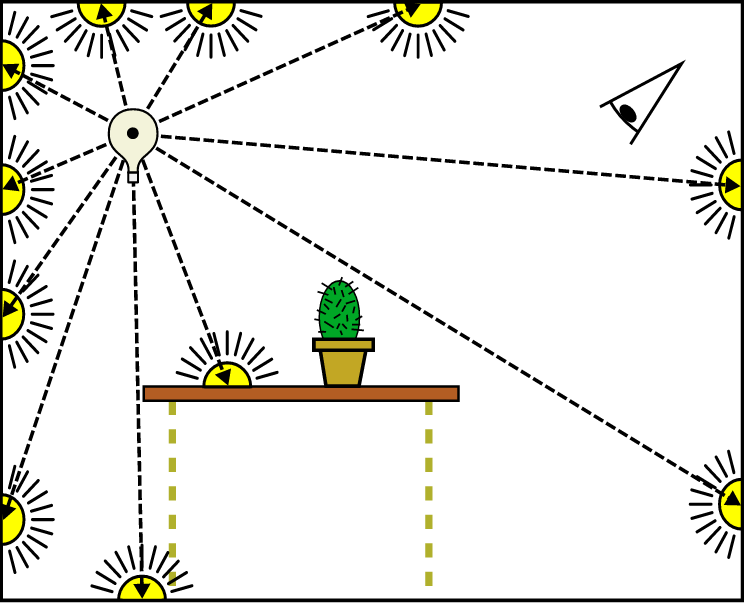
\includegraphics[width=.48\textwidth]{graphics/many_lights_laine_1} &
    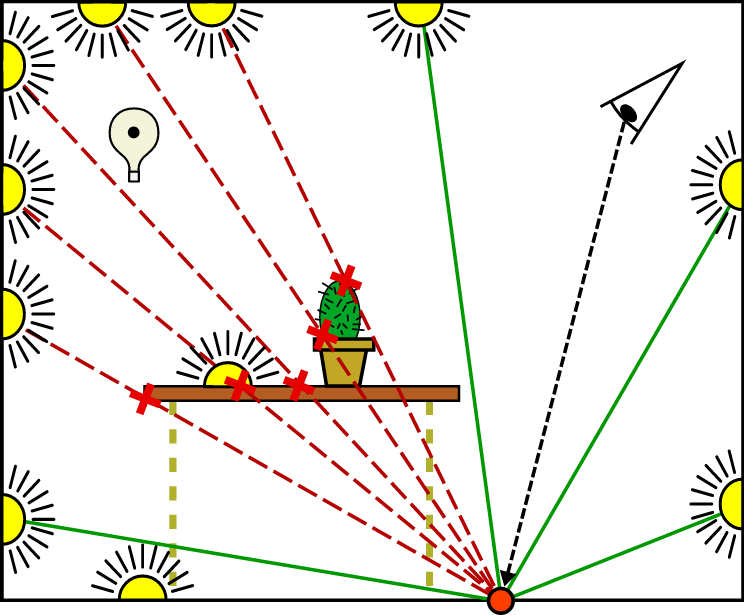
\includegraphics[width=.48\textwidth]{graphics/many_lights_laine_2}\\
  \end{tabular}
  \caption{Illustration of the many-light concept. Left: VPLs are created on surfaces that are directly lit by a light source. Right: When shading a surface point (orange), all VPLs that are visible for that point are used to indirectly light it. Figures reprinted from \citet{laine2007incremental}.}
  \label{fig:intro:many_lights_visualization}
\end{figure}

The use of many-light methods is intriguing since they are a natural and intuitive model of real-world light interactions. In addition the concept is highly scalable: Many-light methods have been used for real-time applications with up to a few thousand lights to offline rendering with millions of lights. Given a sufficient number of lights, the concept is capable of accurately simulating advanced effects like subsurface scattering and participating media. \citet{Dachsbacher:2014:ManyLightsSTAR} gives an overview of the higher-end spectrum of many-light methods.

When applied to real-time applications, the available performance budget enforces the use of a limited number of lights. With a few thousand lights at most, many effects are not possible to reasonably approximate anymore. However, the low-frequency nature of diffuse reflections enables several approximations and optimizations that make a convincing global illumination effect feasible to create. Using more or less conventional point light sources has another advantage, at least in the context of real-time applications: Many techniques from classical real-time rendering are applicable, such as point light rendering including conventional shadow maps for visibility testing. This allows for simple implementations of the basic concepts, even though more advanced techniques are necessary to achieve high performance and quality levels.



\subsection{Components of Many-Light Methods}
This section will take the components of global illumination identified in \Cref{sec:intro:gi:components} and explain how they translate to many-light methods. Two new components are added that are unique to many-light methods, namely VPL placement and mitigating singularities.

\begin{description}
    \item[Direct lighting or light injection.] In theory, many-light methods do not need a light injection step since they are usually iterative processes that start with the scene lights and from there on, create new lights wherever the current light set illuminates the scene. In practice, the first bounce is often handled separately for performance reasons, and because the VPLs have different characteristics than most scene lights.
    \item[Light propagation.] As just mentioned, many-light methods can simulate an arbitrary number of light bounces by repeating the propagation step with an expanding set of VPLs. However, many techniques (and this thesis) simulate just the first bounce, since that alone provides a large quality enhancement over simulating no global illumination at all, and subsequent bounces are more complex in terms of implementation and computation.
    \item[VPL placement.] Since the budget of VPLs is limited, it is desirable to get the maximum effect out of each VPL. Thus, much research has gone into placing VPLs where they contribute the most to the output image, while at the same time not introducing any bias. Both the light injection and light propagation step create VPLs and can take considerable amounts of computation time through complex sampling methods. Some techniques also do not distinguish between light injection and light propagation and have a unified process for placing VPLs.
    \item[Final gathering.] Most many-light methods perform final gathering per screen-space pixel. There are two main approaches commonly referred to as splatting and gathering. Both are too slow to use every light to shade every pixel, therefore optimizations and approximations are used. More on this in the next section.
    \item[Visibility testing.] Many-light methods provide no means of visibility computation; these need to be solved separately. The advantage of many-light methods is that each receiving element only needs to test the (bounded) number of VPLs for visibility, not an arbitrarily high number of scene elements. In contrast to other global illumination methods, this makes it possible (although not performant) to use shadow maps for visibility testing.
    \item[Choice of receiving elements.] As mentioned before, screen-space pixels are most commonly used, albeit often downscaled or combined with interleaved sampling (\Cref{sec:intro:relatedWorkManyLight:finalGathering}). The other options listed in \Cref{sec:intro:gi:components} are technically possible as well, but haven't been combined with many-light methods yet.
    \item[Mitigating singularities.] Since the entire energy of the indirect light bounces is concentrated into a few infinitely small light sources, the areas near these light sources receive too much light. This effect is distinctly visible as bright spots around the VPL's location (\Cref{fig:introGI:clamping}), making it necessary for many-light methods to alleviate this artifact.
\end{description}

\begin{figure}[htb]
    \centering
    \begin{subfigure}[b]{0.32\textwidth}
        \centering
        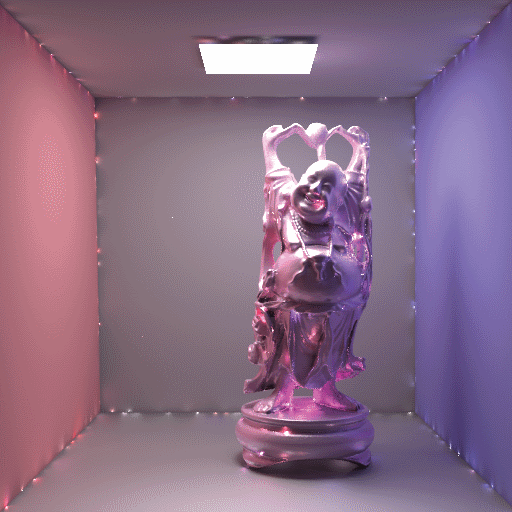
\includegraphics[width=1.0\linewidth]{graphics/clamping1-dachsbacher}%
        \caption{}
    \end{subfigure}%
    \hfill
    \begin{subfigure}[b]{0.32\textwidth}
        \centering
        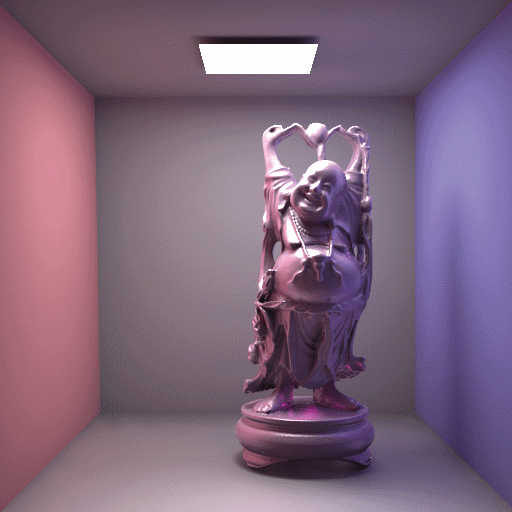
\includegraphics[width=1.0\linewidth]{graphics/clamping2-dachsbacher}%
        \caption{}
    \end{subfigure}%
    \hfill
    \begin{subfigure}[b]{0.32\textwidth}
        \centering
        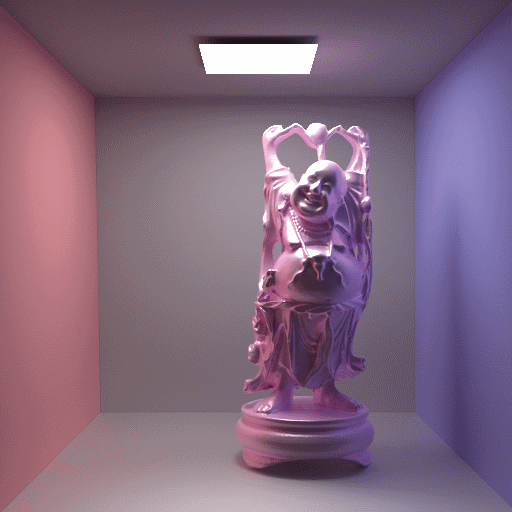
\includegraphics[width=1.0\linewidth]{graphics/clamping3-dachsbacher}%
        \caption{}
    \end{subfigure}%
    \caption{A rendering generated using a many-light method. (a) Naive approaches produce singularities near the VPL's location. (b) Clamping the light attenuation term makes the problem less apparent, but causes bias in the form of darkening in the corners and on the statue. (c) An unbiased rendering for comparison. Figure reprinted from \citet{Dachsbacher:2014:ManyLightsSTAR}.}
    \label{fig:introGI:clamping}%
\end{figure}%



\section{Previous Work on Real-Time Many-Light Methods}
\label{sec:intro:relatedWorkManyLight}

This section will present several many-light methods while concentrating on those that are applicable to real-time rendering. It is structured roughly according to the different design decisions to be taken when applying many-light methods: VPL sampling, computing visibility, final gathering, and mitigating singularities. The light transport step is not covered separately as it is often either omitted, simulating only one bounce, or it is an integral part of the VPL sampling algorithm. The choice of receiving elements is not covered as well, as most papers in this area simply use screen-space pixels. \citet{Dachsbacher:2014:ManyLightsSTAR} provide another overview of many-light methods, including those unsuitable for real-time rendering.


\subsection{Virtual Point Light Sampling}
\label{sec:intro:relatedWorkManyLight:vplSampling}

While \citet{Keller:1997:InstantRadiosity} proposes an approach similar to photon mapping to create VPLs, real-time applications are in need of something more performant. A commonly used technique are \emph{reflective shadow maps} (RSMs, \cite{Dachsbacher:2005:RSM}), which use rasterization to create first-order VPLs. While in this paper, each pixel of the RSM is considered a VPL and during gathering, a random subset of all VPLs is sampled, beginning with \citet{dachsbacher2006splatting} most papers sample the RSM to create a fixed set of VPLs which is used during shading.

\citet{georgiev2010simple, ritschel2011ismsViewAdaptive} sample the RSM to create a set of VPLs with (estimated) high contributions to the final image. \citet{dong2009real, prutkin2012reflective} cluster several samples to form \emph{virtual area lights}. They observe that far fewer virtual area lights than VPLs are necessary to achieve the same quality at a minor performance expense.

Most of these approaches suffer from poor temporal stability. To improve on that, \citet{laine2007incremental} update only a portion of the VPLs per frame but introduce latency to the indirect light, additionally dynamic objects can receive but not bounce light. \citet{barak2013temporally} provide temporally stable results with dynamic scene geometry, but not with moving light sources. \citet{hedman2016sequential} achieve near-optimal temporal stability even with moving light sources while maintaining high per-image accuracy at real-time frame rates. They use one classic shadow map per VPL though, which must be updated lazily to stay within real-time limits.


\subsection{Final Gathering}
\label{sec:intro:relatedWorkManyLight:finalGathering}

Splatting techniques have been used to add a light's contribution to the rendered image \citep{dachsbacher2006splatting, Nichols:2009:splatting}, but do not utilize modern GPUs efficiently. Instead, gathering approaches are commonly used today, employing interleaved sampling \citep{Keller:2001:InterleavedSampling} to reduce the number of lights processed per pixel, in combination with an edge-aware blur similar to \citet{laine2007incremental}. \citet{segovia2006non} improve the cache efficiency of interleaved sampling.


\subsection{Visibility Computation}
\label{sec:intro:relatedWorkManyLight:visibility}

There are several approaches to calculate visibility between VPLs and the scene parts visible to the camera. Classic shadow maps are a fairly exact solution, but cannot be updated every frame for the several hundreds or even thousands of VPLs.

A popular approach are \emph{imperfect shadow maps} \citep[ISMs,][]{ritschel2008ism}, which use a precomputed set of points as scene representation to quickly render large amounts of small and inaccurate shadow maps. \citet{ritschel2011ismsViewAdaptive} extend the approach to fully dynamic scenes among other improvements. \citet{barak2013temporally} use tessellation to compute the point set, eliminating the need to keep a separate point set updated, making it inherently dynamic, and providing better performance for larger point sets.

Ray tracing has been proposed to compute visibility as well \citep[e.\,g.,][]{segovia2006bidirectional}, but suffers from the usual drawbacks of ray tracing in a real-time context. A voxel-based scene representation has also been used to perform visibility queries for many-light techniques \citep{sun2015manylightsSVO}.


\subsection{Mitigating Singularities}
\label{sec:intro:relatedWorkManyLight:singularities}

In naive implementations of many-light techniques, bright spots will appear near the VPL’s positions due to the light’s attenuation term approaching infinity. A common approach is to clamp the term (\Cref{fig:introGI:clamping}). This introduces bias, which can be compensated, e.\,g., in screen space \citep{novak2011screen}. Singularities can also be avoided through more advanced light representations \citep{tokuyoshi2015vsgl}.


\cleardoublepage

%!TEX root = foo-thesis.tex

\chapter{Concept}

\section{Global Illumination Pipeline Overview}
\label{sec:concept:overview}

\begin{figure}[h]
    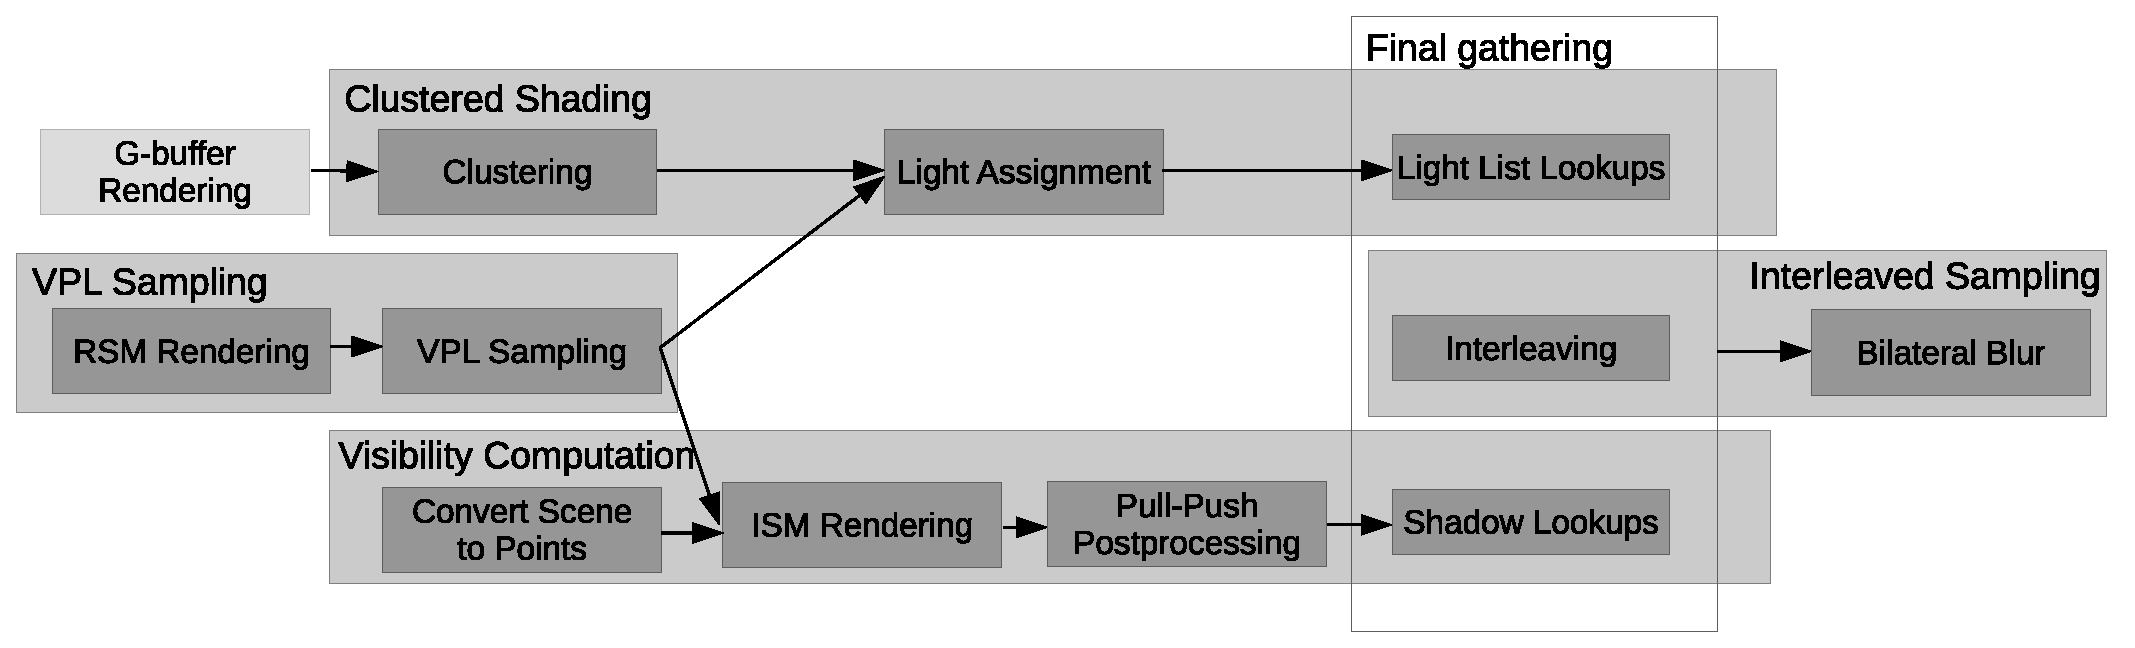
\includegraphics[width=\textwidth]{graphics/GI_pipeline_concept_rough}
    \caption{Global Illumination pipeline concept.}
    \label{fig:GIPipelineConcept}
\end{figure}


This chapter will detail the individual stages of the global illumination pipeline presented in this thesis. Figure~\ref{fig:GIPipelineConcept} provides an overview.
The reflective shadow map and the subsequent VPL sampling (left part of middle row in the diagram) will be covered in the following section.
Section~\ref{sec:concept:ism} describes the rendering process for the imperfect shadow maps (lower row) in detail.
The final gathering step uses data from the clustered shading technique (upper row, detailed in Section~\ref{sec:concept:clusteredShading}) and performs interleaved sampling (right part of middle row, detailed in Section~\ref{sec:concept:interleavedSampling}).
Finally, during final gathering, we use clamping to remove singularities, this is shortly presented in Section~\ref{sec:concept:clamping}.
Our G-buffer rendering does not differ from common deferred rendering pipelines and is not covered further.


\section{Virtual Point Light Sampling with Reflective Shadow Maps}
\label{sec:concept:rsmVplSampling}

VPL sampling has not been the focus of this thesis, therefore we use a rather basic approach by rendering a  simple reflective shadow map and regularly sampling it. \citet{hedman2016sequential} present a more advanced approach.

\begin{outline}
\1 Often preferred due to the simplicity and speed because rasterization. but, first bounce only.

\1 Similar to regular G-Buffer rendering

\1 Like shadowmaps, scene is rendered from the light's viewpoint

\1 Unlike shadowmaps, not only depth is rendered but additionally normal and (diffuse) surface color.

\1 The result can be sampled to create VPLs with a certain position reconstructed from the depth buffer, and normal and color taken from the additional buffers.

\1 In our case, we use regular sampling. Importance-based approaches are available, also the samples can be clustered \cite{} or chosen relative to their estimated contribution to the final output. \citet{hedman2016sequential} uses a different approach without RSMs.

\end{outline}

\section{Visibility Computation with Imperfect Shadow Maps}
\label{sec:concept:ism}


The original paper \citep{ritschel2008ism} converts the scene geometry to a point set in a preprocessing step and uses the points to efficiently render hundreds of shadow maps in parallel. They use splatting to render the points and fill the resulting holes in the shadowmaps with a pull-push algorithm inspired by \citep{Marroquim:2007:reconstruction}.

\citet{ritschel2011ismsViewAdaptive} build on this by converting the scene to a triangle texture dynamically, and sampling the points from that texture. Instead of computing a triangle texture, \citet{barak2013temporally} use the tessellation units of recent GPUs to dynamically convert triangles into points.
We follow this approach since it is relatively simple to implement and inherently dynamic, but have not implemented the adaptive sampling from \citet{ritschel2011ismsViewAdaptive} yet.
\citet{ritschel2008ism} also present multi-bounce indirect illumination with their technique, which we have not implemented.
We describe the point rendering process in the following section and subsequently detail the pull-push algorithm.

\subsection{Point Rendering with Splatting}
\begin{outline}
\1 render the scene
\1 depending on the size of the triangle, set tessellation levels
\1 of the resulting tessellated triangles, take the center, calculate approx world size of disk
\1 while it might be faster to just use the vertices as points, we take the center of each triangle to be more accurate, otherwise the points on the edge of the triangle will enlarge the rendered area considerably.
\1 pick a random VPL, perform culling, render splat into the VPL's ISM. To simplify the calculations, the ISM uses a paraboloid mapping. Here another advantage of the points comes into play: Compared to triangles it is trivial to perform a paraboloid projection for points.
\1 As an optimization, we iterate over several VPLS, and collect some that pass the culling test, and render to those. more in implementation chapter
\1 To remove holes in the resulting shadowmap, the original paper implements a simplified variant of \citet{Marroquim:2007:reconstruction} that only uses depth information from the point rendering. We found that this approach has little benefit over simply enlarging all the point splats during rendering, therefore we did not use it when using splat rendering.
\end{outline}

\subsection{Point Rendering with Pull-Push Postprocessing}

\begin{outline}
\1 Besides point splat rendering, we also pursued a second approach that follows the algorithm of \citet{Marroquim:2007:reconstruction} more closely with the intent to obtain higher-quality shadowmaps. More specifically points are rendered as a single pixel, albeit with additional attributes like size and normal. These are then used in a subsequent reconstruction pass to create an (ideally) hole-free shadowmap. This approach also allowed a point to be rendered into multiple shadowmaps with a moderate performance impact, more on this in the next chapter.

\1 rough overview: the algorithm is a ``pyramid-method'' and uses miplevels.
\1 a pull phase aggregates the information from four pixels of a finer level to one pixel of a coarser level.
\1 a subsequent push phase aggregate four pixels of a coarser level to one pixel of a finer level if the pixel of the finer level contains no data or is determined to belong to an occluded surface. This way, closed surfaces are derived from single-pixel points.

\1 Pull phase
    \2 It only considers pixels that pass the following tests: First, they need to contain a valid depth at all (i.e. a point must have been rendered into this pixel) and second, the pixels depth must not be greater than the frontmost of the four considered pixels plus its depth interval. If this test fails, the point is assumed to belong to a different surface that is occluded and thus should not be used for interpolation.
    \2 The depth interval of each point is determined by adding a constant value to the rendered depth for the points in the lowest miplevel. For interpolated points, the new depth interval spans the calculated depth of the point to the highest depth value of the depth intervals of all points used for aggregation.
    \2 The depth and radius attributes are interpolated in between with equal weights. Since the center of the aggregated point might not match with the position of the pixel (this happens if not all four pixels are used for interpolation), a displacement vector is also calculated that describes the point's location.
\1 Push phase
    \2 Again only pixels that pass certain tests
        \3 Analogous to the pull phase, points must contain a valid depth and not be occluded.
        \3 A radius check: If the pixel's location is outside the point's extends described by the displacement vector and its radius, then the point is not considered either. This is done to limit a point's influence to its actual size.
    \2 The pixel of the finer level might already contain data computed during the pull phase. This data is overwritten if the aggregated data has a smaller depth, i.e. if the original data is considered to be occluded. Otherwise, the original point is left as it is.
    \2 The weights used for interpolation during the push phase are not uniform, see Figure~\ref{fig:???}.
\1 \citet{Marroquim:2007:reconstruction} also use the point's normals to correctly limit the point's size, and \citet{Marroquim:2008:reconstruction2} propose gaussian weights based on the pixel's distance to the point's location, instead constant weights solely based on pixel locations. Both of these additions we have not implemented yet.
\end{outline}



\section{Clustered Deferred Shading}
\label{sec:concept:clusteredShading}

In real-time graphics applications, primarily video games, a technique called \textit{clustered shading} \citep{olsson2012clustered}, has seen increased usage. Its goal is to increase the efficiency of lighting a scene with multiple light sources.
The effectiveness of clustered shading in the context of many-light global illumination has not been studied so far to our knowledge, and we aim to contribute a few datapoints to this end.

The integrated algorithm works as follows:
\begin{outline}
\1 view frustum is divided into a fixed number of clusters
\1 for each fragment, determine cluster. clusters with no fragments are ignored.
\1 for each cluster, determine the VPLs that can reach that cluster, put into light list.
\1 during shading, don't iterate over all VPLs but only those from the light list.
\1 usually, large benefits due to limited radius. we have infinite radius, but at least we can discard half the lights because hemisphere.
\1 As an extension, \citet{olsson2012clustered} propose to calculate explicit bounds for the cluster's fragments to enable more precise culling. we expected only moderate performance gains from that and have not implemented it.
\1 Another extension is to use the surface normal's direction as fourth dimension after the three spatial dimensions for clustering, allowing for some sort of backface culling for even greater efficiency. While this seems more promising in terms of performance gains, we have not implemented it either (wir sind bisher nicht dazu gekommen).
\end{outline}

Clustered shading is an extension and improvement to \textit{tiled shading} \citep{Olsson:2011:TiledShading}, that uses screen-space tiles instead of view-space clusters. Tiled shading has previously combined with many-lights global illumination by \citet{Tokuyoshi:2016:Stochastic}. They use an order of magnitude more lights than we do, but stochastically limit them in range. As a result, the light culling is much more effective in their case.
We implement tiled shading as well and compare it to clustered shading.


\section{Interleaved Sampling}
\label{sec:concept:interleavedSampling}
Interleaved sampling \citep{Keller:2001:InterleavedSampling} is often used to vastly improve the performance impact of GI methods.

\begin{outline}
\1 general idea: given some amount of samples that, in a naïve implementation, would be performed per pixel, distribute those samples over a 4x4 or 8x8 block of pixel
\1 the naïve implementation hurts cache coherency, since adjacent pixels process different samples.
\1 to this end, de-interleaving \citep{segovia2006non} is often used to simultaneously process those pixels that use the same sample set. see Section~\ref{sec:impl:interleavedShading} for details.

\1 results in structured noise and missing information as all pixels have only part of the samples
\1 therefore, geometry-aware blur similar to \citet{laine2007incremental} to distribute the information
\1 the blur is separated (although since it is a bilateral filter, this is mathematically not equivalent, but difference is not noticeable), linear filter, and uses world-space distance and dot product between the samples as weight

\1 all this works because low-frequency effect

\1 In most aspects we follow this standard approach. The only notable deviation is our implementation of de-interleaving that does not use any separate splitting/merging passes, again we defer details to Section~\ref{sec:impl:interleavedShading}.

\end{outline}



\section{Removing Lighting Singularities through Clamping}
\label{sec:concept:clamping}
It's simple, we clamp the singularities. Wouldn't be necessary with infinite number of lights. \citet{hedman2016sequential} reach high accuracy even with clamping and 2k lights.

%!TEX root = foo-thesis.tex


\chapter{Implementation}

\section{Used Libraries and the Framework gloperate}

\todo[color=green]{software architecture?}

- some architecture diagram of dependencies?
- gloperate as framework
    - uses qt
- libzeug provides GUI elements
- globjects as an object-oriented abstraction over OpenGL
- glbinding provides OpenGL bindings, directly called sometimes
- GLM provides math and easier interaction with the OpenGL API
- no further relevance for this thesis:
    - assimp for model loading
    - glkernel provides kernels for our SSAO implementation
    - cpplocate ???

\section{Rendering Pipeline Overview}
- would be much the same as the concept pipeline...
- show what's compute shader and what not?
- it's basically lighting plus
    - g-buffer generation
    - shadowmap which is part of the RSM,
    - SSAO
    - deferredshading
    - srgb and HDR.
    - all of this is not
- model loading?
- kernel generation?


\section{RSM Generation and VPL Sampling}
\label{sec:impl:rsmAndVplSampling}
- use the same code for RSM generation as for G-Buffer generation with only slight modifications:
- don't use normalmaps as the triangle normals are sufficient
- instead of individual texture lookups, we use the material's average color as diffuse color as suggested by \citet{hedman2016sequential} to avoid high-frequency color changes to affect the outcome.
- we re-use RSM as shadowmap
    - usually, one might want to decouple this since they likely need different resolutions/cascading schemes etc. One could also render the RSM with a less detailed version of the scene. Since we had no culling and LOD implemented, we were bottlenecked on geometry complexity and chose to do this in one pass.
    - we use variance shadowmapping. so we add the variance buffer if we're rendering an RSM, and disable another buffer (non-face normals).

- with a compute shader, we sample the RSM in a regular pattern and write VPLs into a buffer
- VPLs are position, normal, color
- we prepare a second buffer with a single vec4 with position in the first three values and normal packed into the last value.
- we do that since the ISM rendering (Section~\ref{sec:impl:ismRendering}) and light list calculation (Section~\ref{sec:impl:clusteredShading}) do not need color and especially ISM rendering reads several VPLs per point, using a lot of bandwidth.
- Because of the regular sampling, the noise produced during interleaved shading (Section~\ref{sec:impl:interleavedShading} or only results? there was a paper that sorts VPLs to avoid the noise...) is more structured. To help with that, we permutate the VPL order with a random permutation computed on CPU

\section{ISM Rendering}
\label{sec:impl:ismRendering}
- Our ISM rendering normally draws all the geometry in the scene.
- In the tessellation control shader, the tesselation levels are determined depending on the triangle size.
- The tessellation evaluation shader does nothing besides correctly interpolating the triangle's vertices.
- The geometry shader, which now recieves a small (tesselated) triangle, computes the point data
- i.e. position: center of triangle, radius: distance of center to farthest triangle vertex, normal: the face normal taken from the original, non-tessellated triangle.

- the geometry shader then calculates a random VPL ID. We used the point's barycentric coordinate inside its triangle and the triangle's primitive ID to seed the random number generator, as both values are readily available and coherent between frames.

- two approaches:

- either the geometry shader itself reads the VPL with the index it determined, projects the point according to the VPL's data, sets gl\_PointSize to the projected size, and emits a vertex.
- also, output mode is points.

- \citet{Marroquim:2007:reconstruction} actually works with single-pixel ``splats''. since in this case we're not depending on the hardware rasterizer for good performance, this inspired the following approach:

- instead of splatting, the geometry shader puts points into buffer
- one buffer per VPL for stability
- buffers index marks the first VPL to try
- then, per point in each buffer, starting with the respective VPL, we test a fixed number of VPLs (e.\,g. 16) and collect up to 4 that pass culling tests.
- specifically, backface culling and points that are located behind the VPL, i.\,e. not in the hemisphere pointing along the VPL's normal.
- we then render the point as a single pixel into the 4 collected VPLs.

\todo{part of this into concept}


- hole mitigation
- when splatting, the quality difference improvement achieved with an additional pull-push algorithm compared to slightly larger splats seemed not worth the performance impact, therefore we chose to simply enlarge all splats a bit.
- when using compute shaders, we need pull-push by design.

\todo{explain pullpush implementation}

\section{Interleaved Shading with Compute Shaders}
\label{sec:impl:interleavedShading}
- often, de-interleaving is implemented by splitting the G-buffer into several smaller G-buffers, each containing all pixels with the same sample set \cite{segovia2006non}. Each G-buffer is processed with its respective sample set, and then the buffers are re-interleaved into a large G-Buffer again.

- instead, we do this in a single pass. compute shaders are launched so that each invocation processes one pixel, and invocations within a work group process the same VPL set.
- \ref{lst:???}?
- diagram of the pixels. \ref{fig:impl:pixels} explain this. we still do coherent VPL processing.
- more explanation on id calculation
- reasons for single pass? easier to implement. latency covering? less bandwidth? less memory. compared to interleaving via shared memory, occupancy and scales to 8x8.
- potential downside is the scattered read compared to coherent read when doing the split. but, bottleneck is lookups in the VPL buffer and the respective shadowmaps in the main loop, as well as ALU operations, so this noe-time lookup doesn't have any impact. maybe completely latency covered or workgroups are distributed in a way that the reads are still cache-coherent.
- in fact, any attempts to do coherent reads did not result in speedups.

- Since only a subset of all samples is processed per pixel and this subset repeats every four pixels, this process results in structured noise (see Figure \ref{fig:???} or this figure in concept?)
- therefore, geometry-aware blur similar to \citet{laine2007incremental}. doesn't smooth over edges. See code snippet \ref{listing:???}. every pixel has all the information now ideally.

- VPL shuffling helps a great deal! See Figure \ref{fig:impl:shuffling}

\section{Clustered Deferred Shading}
\label{sec:impl:clusteredShading}


- we use 128 pixels as screen-space tile width and 16 depth slices. We also use an optimization proposed by \citet{persson::2013::practical} and use a larger near cluster for better depth slice utilization.

- we do not use explicit bounds, since we expect only small gains by that. although it might result in larger gains, we have have not implemented using normals for clustering yet.
- \citet{???practical} do culling on the CPU. they have small radii and can therefore quickly determine the clusters that are reached by a certain light.
- we have infinite light radii and therefore lots of clusters per light. therefore, we can expect to cull maybe half the lights and not the majority.
- therefore, we decided to iterate over all lights per used cluster, as opposed to iterate over reached clusters per light.
- the more uniform control flow of this approach as also better suited to GPUs.


- three phases, each corresponding to one dispatch compute call:
    - clustering
        - each work group processes one tile and has one 16 bool array which indicates which depth slices in that tile are used.
        - for each fragment, set the corresponding bool to true. no synchronization needed.
        - since the work group size is limited, we set it to 128 and let each invocation iterate through 128 pixels in the tile to cover all pixels.
        - per work group, count the number of used slices
            - we use the first 16 threads in the work group and atomic adds, but one could just as well let one thread do it serially, it doesn't matter.
        - then it adds the number of used depth slices to one global atomic counter. the glsl function to do this returns the value of the counter before the addition.
        - this way, each workgroup ``allocates'' some space in the list of used clusters. it then writes an id for each cluster into that list.
    - calculating light lists
        - one invocation per used cluster.
        - calculate world-space corners of that cluster.
        - show some code? but it's really ugly...
        - for each light
            - if any corner is inside the illuminated hemisphere, add the light to this cluster's light list.
        - we simply allocate the maximum space for this.
            - for full HD / 128px tiles = 135 tiles, * 16 depth slices = 2160 light lists, * 1024 vpls = 2160k indices, * 2 bytes per index makes 4mb.
            - we thought it's unneccessary to cut that down.
            - by a (conservative) estimate of four used depth slices per tile on average, (plus possibly runtime checks to allocate more space when running over that limit), on could reduce this to 1MB with little implementation effort.
            - compacting the light lists themselves is probably not worth it due to implementation complexity and performance penalty
            - since we expect to cull roughly half the lights, the potential saving by compacting the light lists is only 50\% anyways.
    - shading
        - during shading, when processing a pixel, the pixel's cluster is first determined and only the lights of this cluster's light list are processed.
        - we use a very basic approach to combine this with interleaved shading: of all lights in the light list, each pixels gets an equally sized fraction. while this might lead to adjacent pixels processing overlapping sets of lights if they are in different clusters, they are either in clusters near to each other in which case the light lists are probably quite similar, or they are in clusters seperated from each other so the geometry-aware blur wouldn't consider them anyway.

%!TEX root = foo-thesis.tex


\chapter{Results and Discussion}
\label{chap:results}

This chapter details the performance and quality characteristics of the implemented techniques and  examines their memory usage. For each technique, it will subsequently discuss the up- and downsides and identify alternatives.

\section{Scenes, Settings and Testing System}
\label{sec:results:settings}

The implementation is tested in the Crytek Sponza and San Miguel scene, with 260k and 7.9M triangles respectively, both provided by \citet{McGuire2011Data}. Unless otherwise noted, the parameters used for the measurements and screenshots are:
\begin{outline}
    \1 1920x1080\,px output resolution
    \1 1024 VPLs
    \1 2048\,px² ISM texture, i.\,e., 64\,px² per ISM
    \1 Single-pixel point renderer enabled, 16 VPLs considered per point, up to 4 collected
    \1 4x4 interleaving pattern
    \1 Clustered shading: 128\,px² tile size, 16 depth slices
\end{outline}

\noindent
The hardware specification of the testing system is as follows:
\begin{outline}
    \1 Intel Xeon W3530 with four cores at 2.8\,Ghz
    \1 NVIDIA GeForce GTX 980 factory-overclocked by ca. 4\%, driver version 375.57
\end{outline}


\section{RSM Generation and VPL Sampling}
\label{sec:results:RsmAndVplSampling}

\begin{figure}[htb]
\centering
  \begin{tabular}{@{}cc@{}}
    \multicolumn{2}{c}{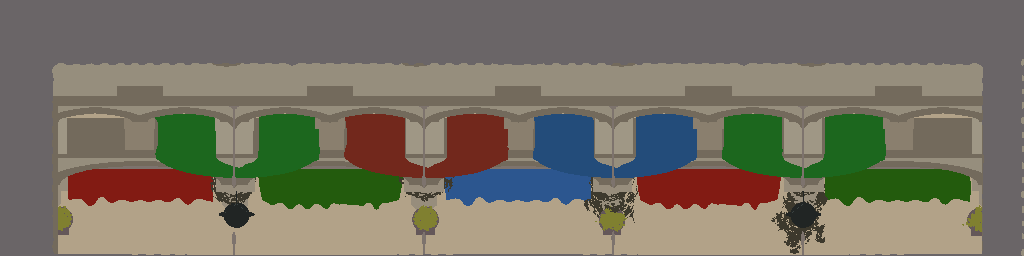
\includegraphics[width=1.0\textwidth]{screenshots/RSM_diffuse}} \\
    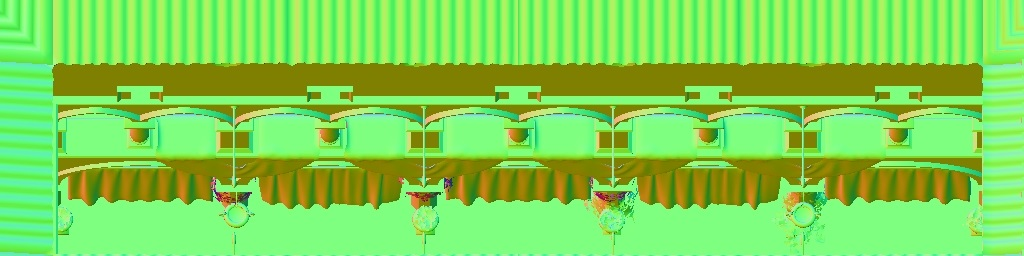
\includegraphics[width=.48\textwidth]{screenshots/RSM_normal} &
    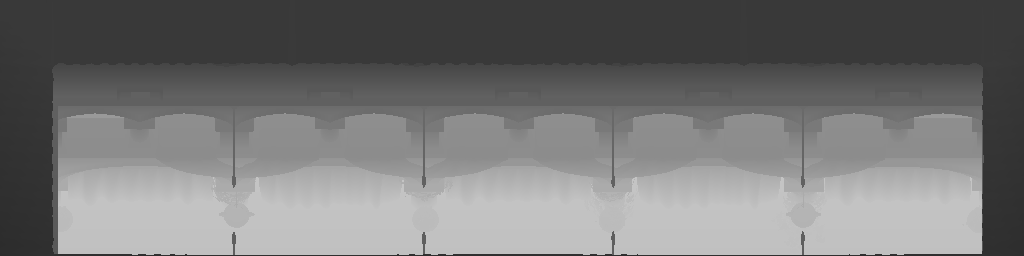
\includegraphics[width=.48\textwidth]{screenshots/RSM_depth}
  \end{tabular}
  \caption{A reflective shadow map, with its diffuse, normal and depth buffer.}
  \label{fig:results:RSMBuffers}
\end{figure}


As explained before, the RSM generation re-uses most of the code of the G-Buffer generation, see \Cref{fig:results:RSMBuffers} for an impression on the rendered result. Accordingly, the performance characteristics are similar to the regular geometry pass of deferred renderers.

Since the implemented VPL sampling distributes the samples over the entire shadow map, we simply limited the VPL's location to the relevant area by tuning the light's extents. As a result, an aspect ratio chosen specifically for each test scene is used.

As our implementation re-uses the RSM as shadow map for direct lighting, we chose a resolution of 512\,px² (or, in the case of the Sponza scene, 1024x256\,px), which is more than required by the naive VPL sampling. The RSM is rendered in 0.17\,ms for the Sponza scene.

The VPL sampling itself takes only several microseconds and is negligible. Bear in mind that, in order to achieve high quality levels, a more elaborate sampling algorithms needs to be implemented, which can actually take most of the available time.

\begin{figure}[htb]
\centering
  \begin{tabular}{@{}c@{}}
    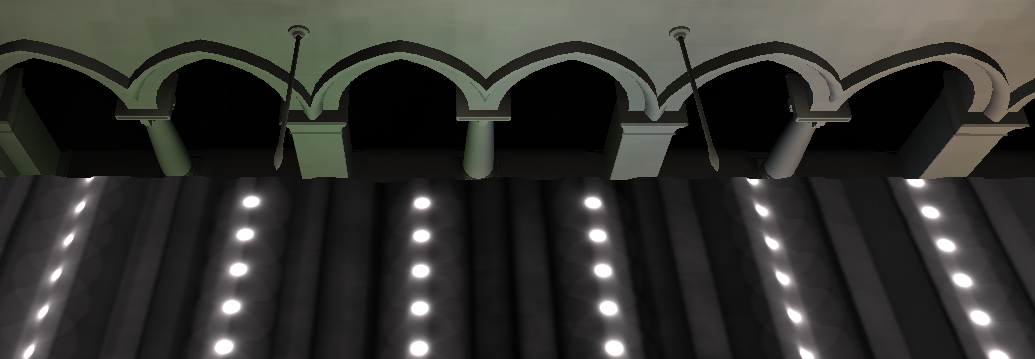
\includegraphics[width=1.0\textwidth]{screenshots/RSM_unfavorable} \\
  \end{tabular}
  \caption{A visualization of inefficiently placed VPLs. Since there is no further geometry above them that could be illuminated, they do not contribute to the final image.}
  \label{fig:results:RSMUnfavorable}
\end{figure}

The sampling does not regard the relevance of the sampled VPLs to the current frame and causes the entire system to be rather inefficient by choosing lights that contribute little or nothing to the rendered output. See \Cref{fig:results:RSMUnfavorable} for an example of unfavorable VPL locations.

An additional downside of the naive sampling is the poor temporal stability when the scene light moves. This is due to each VPL staying at the exact same position in the light's viewport, so it strictly ``follows'' the light's movement, jumping over depth discontinuities along the way. See \Cref{???} for a figure visualizing the frame-to-frame coherency.

\todo{frame-to-frame coherencey screenshots/visualization}


\section{ISM Rendering}

\subsection{Point Rendering with Splatting}




%\Cref{fig:???} shows the Crytek Sponza scene rendered using ISMs created by the splat renderer (a) and the single-pixel renderer (b). A section of the ISM texture is shown for each renderer in the lower row.


\subsubsection{Quality}
\label{sec:results:ism:quality}

\begin{figure}[htb]
\centering
  \begin{tabular}{@{}cc@{}}
    
\includegraphics[width=.48\textwidth]{screenshots/ism_splat_cropped} &
    
\includegraphics[width=.48\textwidth]{screenshots/ism_single_pixel_cropped}
  \end{tabular}
  \caption{ISMs rendered using the splat renderer (left) and single-pixel renderer (right) with default settings. The single-pixel renderer performs interpolation between points, uses more points and does not let points ``bleed'' into neighboring ISMs, but takes more time.}
  \label{fig:results:isms}
\end{figure}

\Cref{fig:results:isms} shows a few ISMs rendered with the splat and single-pixel renderer. The imperfections do show, and not only through the low resolutions. The distortion of the surface silhouettes by the splat renderer or postprocessing contribute their part, making it hard to identify which part of the Crytek Sponza is shown.

\begin{figure}[htb]
\centering
  \begin{tabular}{@{}cc@{}}
    \includegraphics[width=.48\textwidth]{screenshots/darkening_splat} &
    \includegraphics[width=.48\textwidth]{screenshots/darkening_single_pixel}
  \end{tabular}
  \caption{Darkening caused by the splat renderer (left) compared to the single-pixel renderer (right). Note that there is no skylight rendered, which leads to an unnaturally dark upper part in the image even for the single-pixel renderer.}
  \label{fig:results:ismDarkening}
\end{figure}

Comparing the screenshots in \cref{fig:results:ismDarkening}, it becomes apparent that the splat renderer causes visible darkening in the upper part of the image. The reason is likely that the point splats are always oriented towards the camera and do not take the point's normal into account when rendering, amplifying the usual aliasing artifacts of common shadow maps. As a result, any point size larger than one pixel causes surfaces that are not directly facing the camera appear nearer than they actually are when doing shadow lookups in the ISMs. A larger shadow bias could compensate for that but would introduce heavier light leaking. Another possibility is to use the normal to calculate a point's depth per fragment at a potentially high performance cost.

As the single-pixel renderer does not use splats, it does not have this problem. One could say it performs the per-fragment depth calculation implicitly during interpolation in the postprocessing phase.


\begin{figure}[htb]
\centering
  \begin{tabular}{@{}cc@{}}
    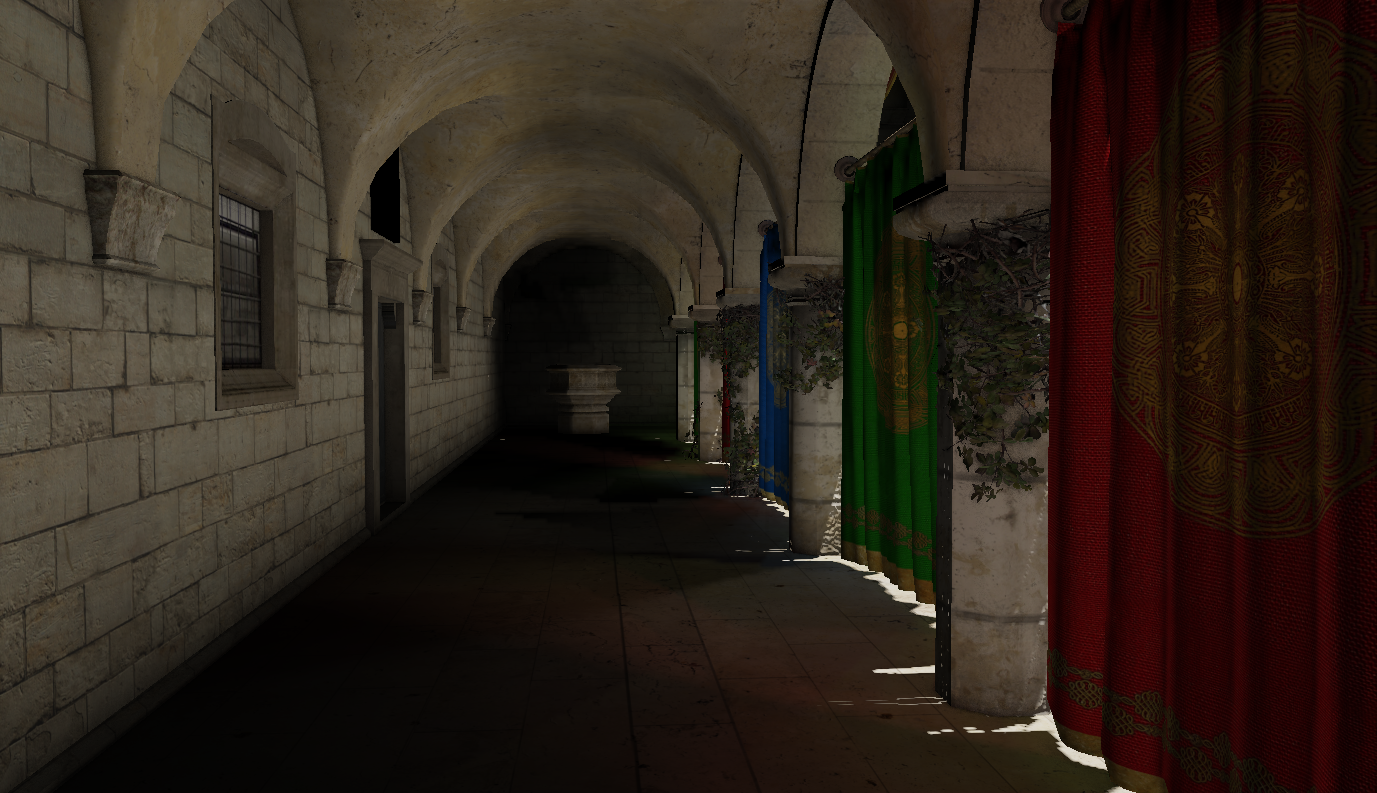
\includegraphics[width=.48\textwidth]{screenshots/leaks_splat} &
    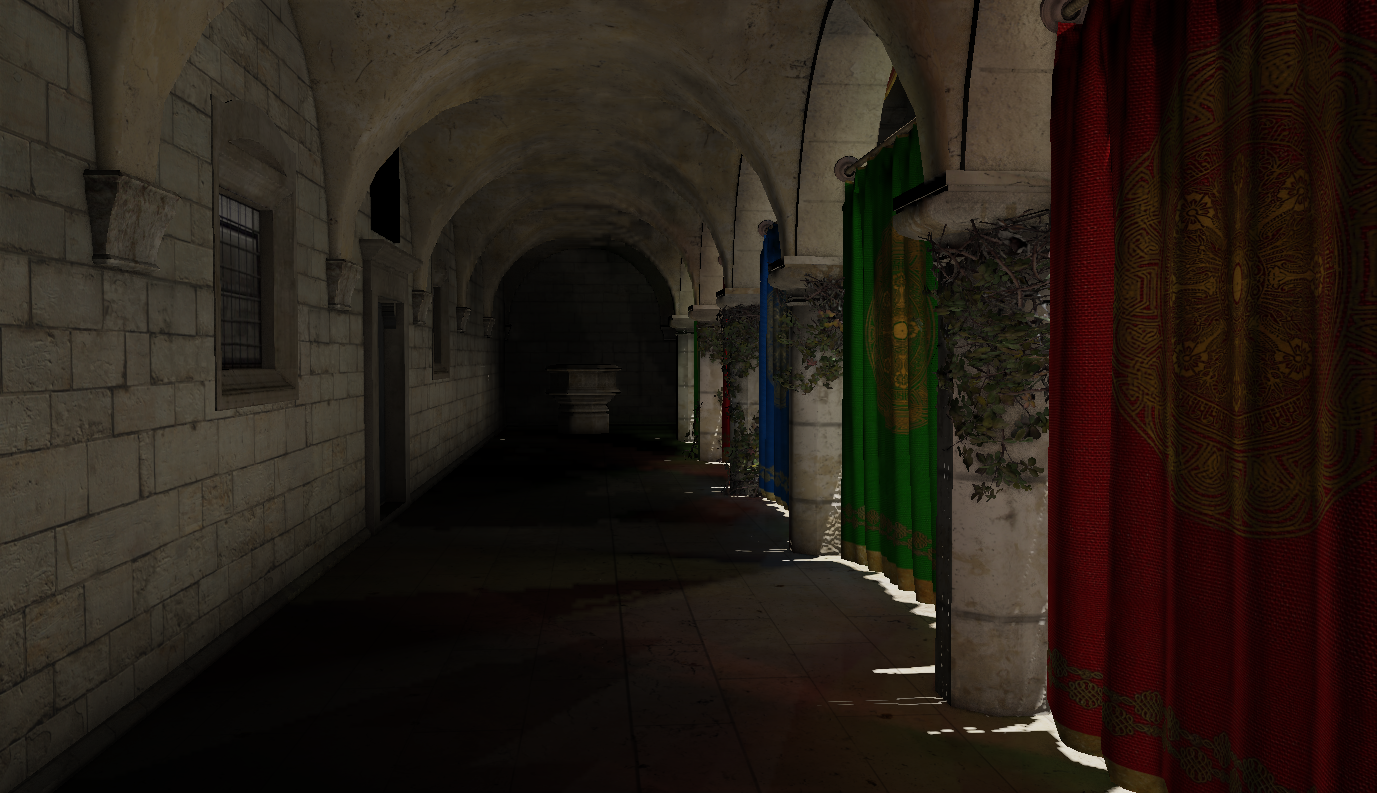
\includegraphics[width=.48\textwidth]{screenshots/leaks_single_pixel}\\
    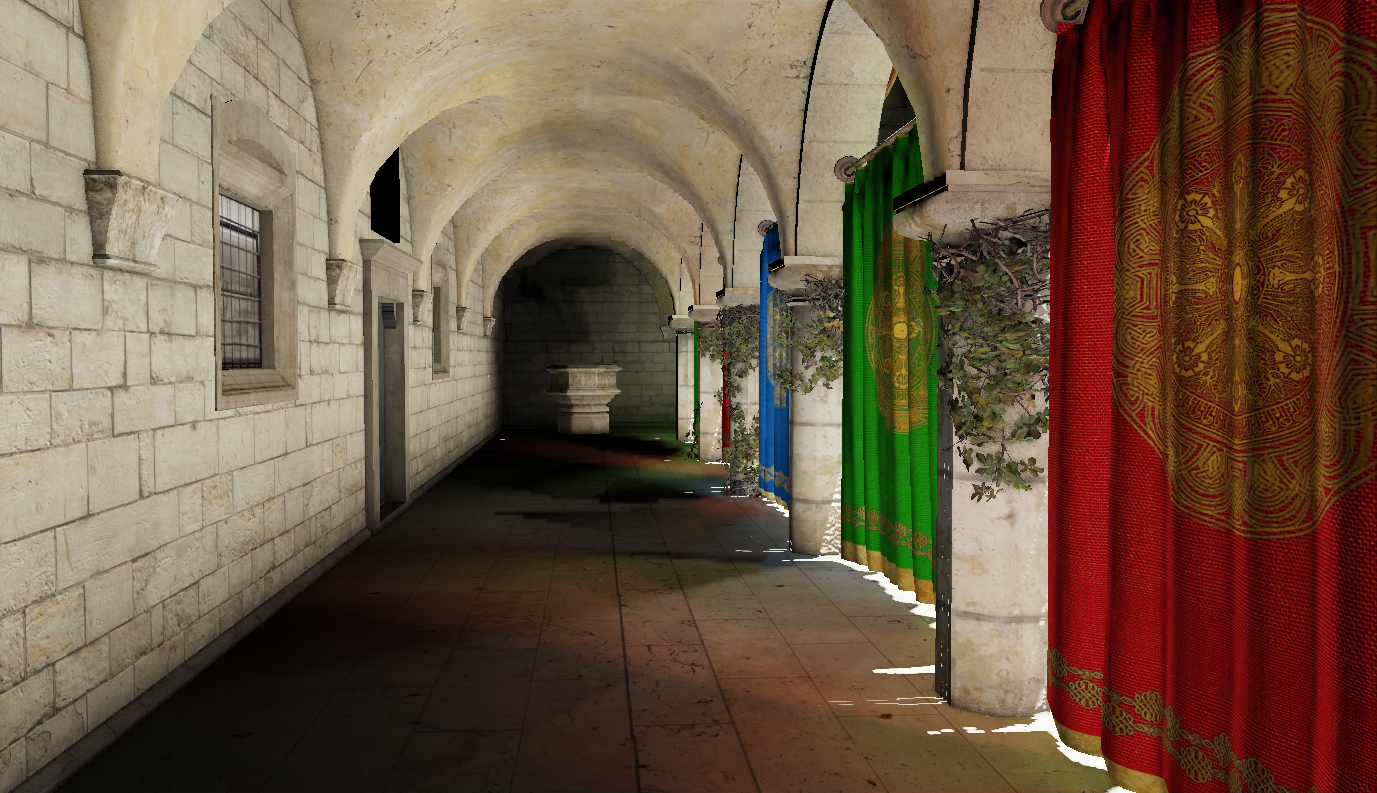
\includegraphics[width=.48\textwidth]{screenshots/leaks_splat_exposure} &
    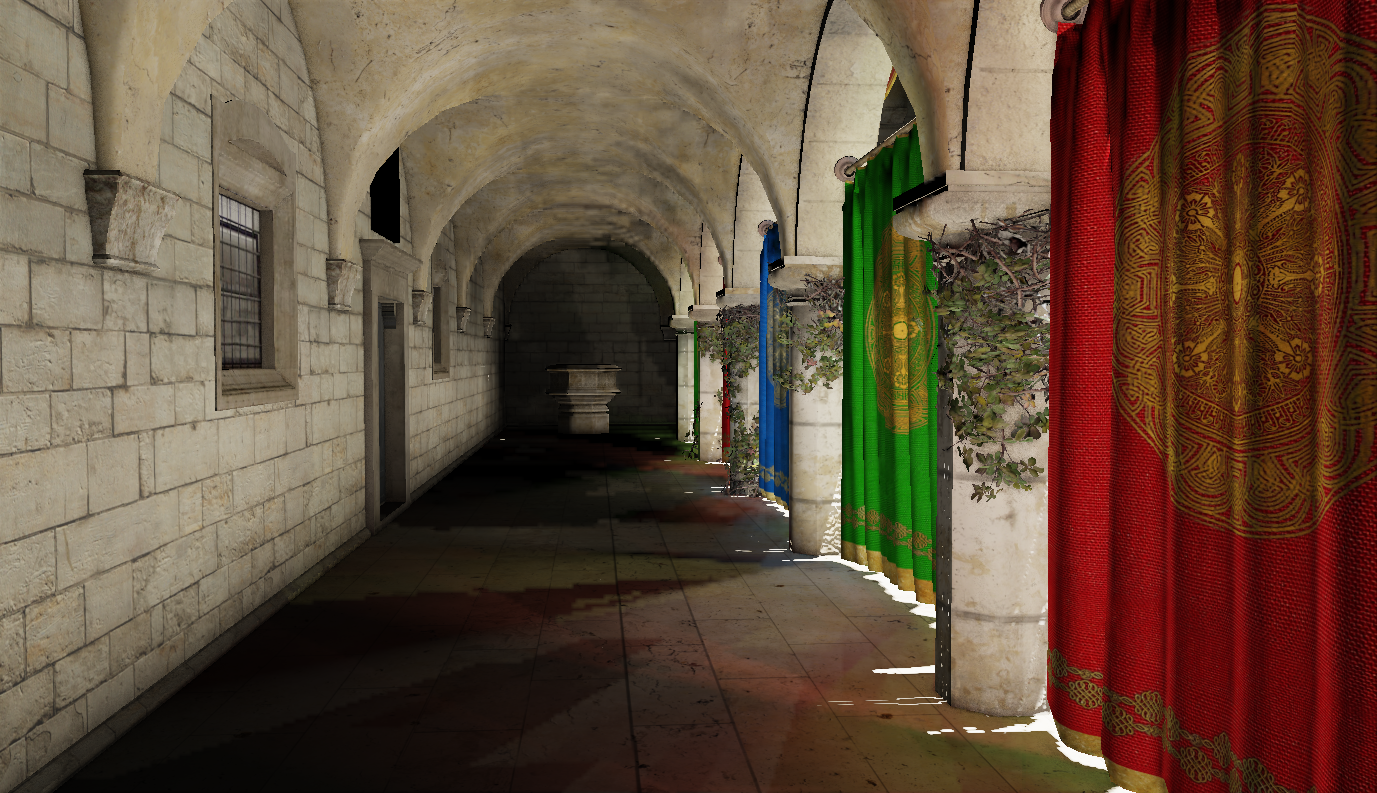
\includegraphics[width=.48\textwidth]{screenshots/leaks_single_pixel_exposure}
  \end{tabular}
  \caption{Light leaks caused by the imperfect shadow maps rendered with the splat renderer (left) and single-pixel renderer (right). VPLs from beneath the curtains leak light onto the wall and ceiling, while VPLs on the pillars and curtains light the floor. The renderings in the bottom row use a higher exposure for illustration. }
  \label{fig:results:leaks}
\end{figure}


\Cref{fig:results:leaks} shows a case the ISM technique has difficulties with. The image should be mostly dark or at least uniformly lit through the small gap below the curtains,instead the wall and ceiling receive a lot of light and the floor displays several artifacts. The root cause is that the VPLs are placed right behind the curtains, so the occluding geometry, i.\,e.\, the curtain, is very near to the light source. Due to the randomness involved when selecting the point set for rendering the ISMs, it often happens that the points near to the light source are rendered into other ISMs, leaving a large hole behind. The single-pixel renderer copes a bit better than the splat renderer since it uses more points, but does not provide a satisfactory result either.



\begin{figure}[htb]
\centering
  \begin{tabular}{@{}cc@{}}
    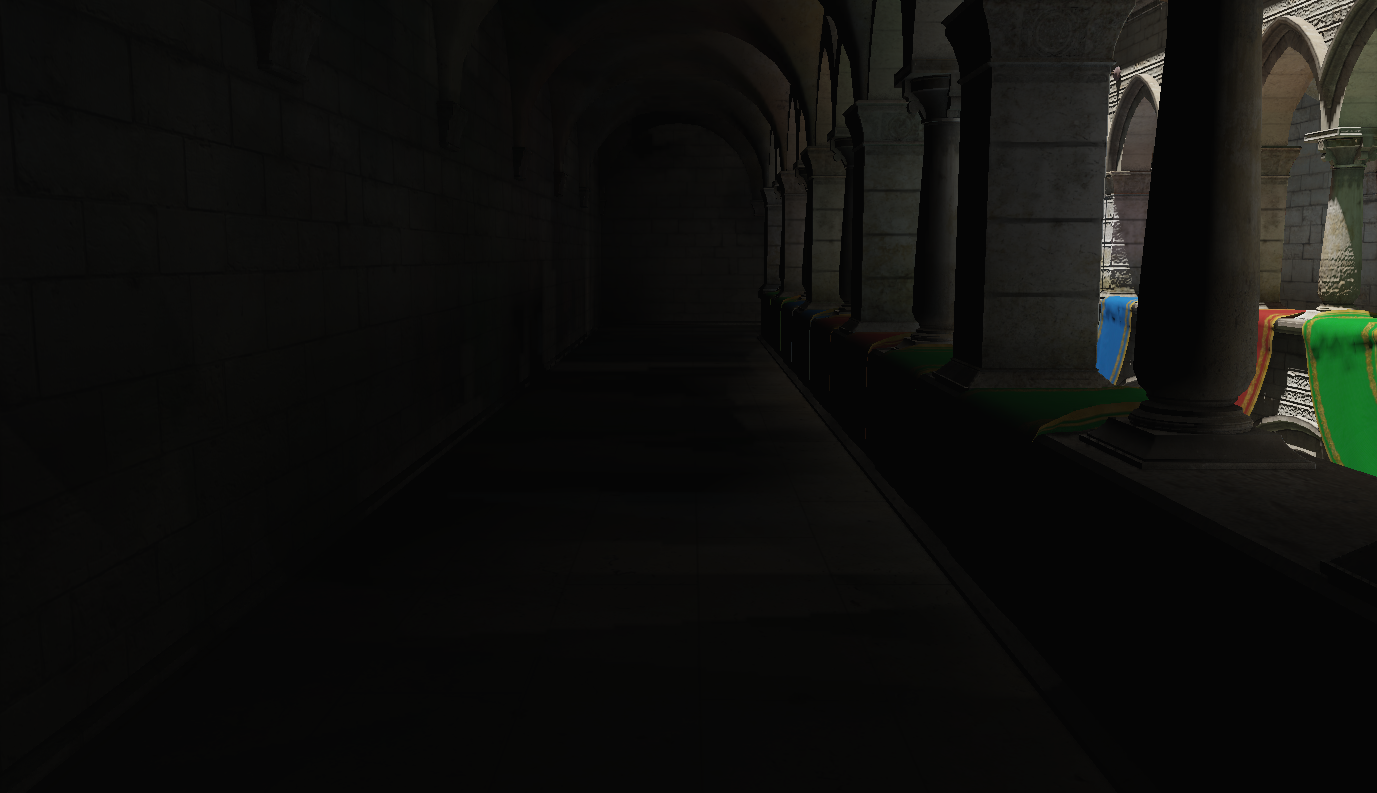
\includegraphics[width=.48\textwidth]{screenshots/bias_splat} &
    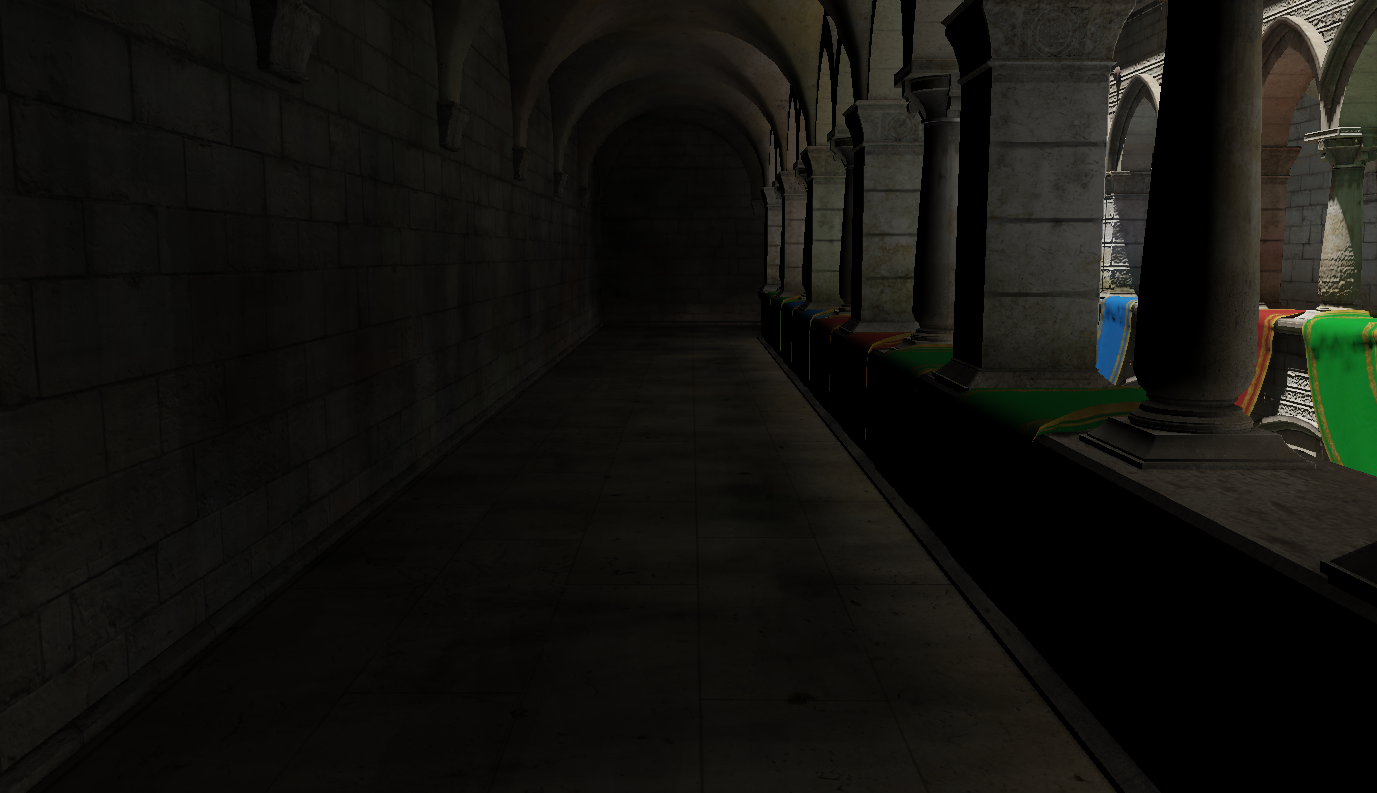
\includegraphics[width=.48\textwidth]{screenshots/bias_single_pixel}\\
      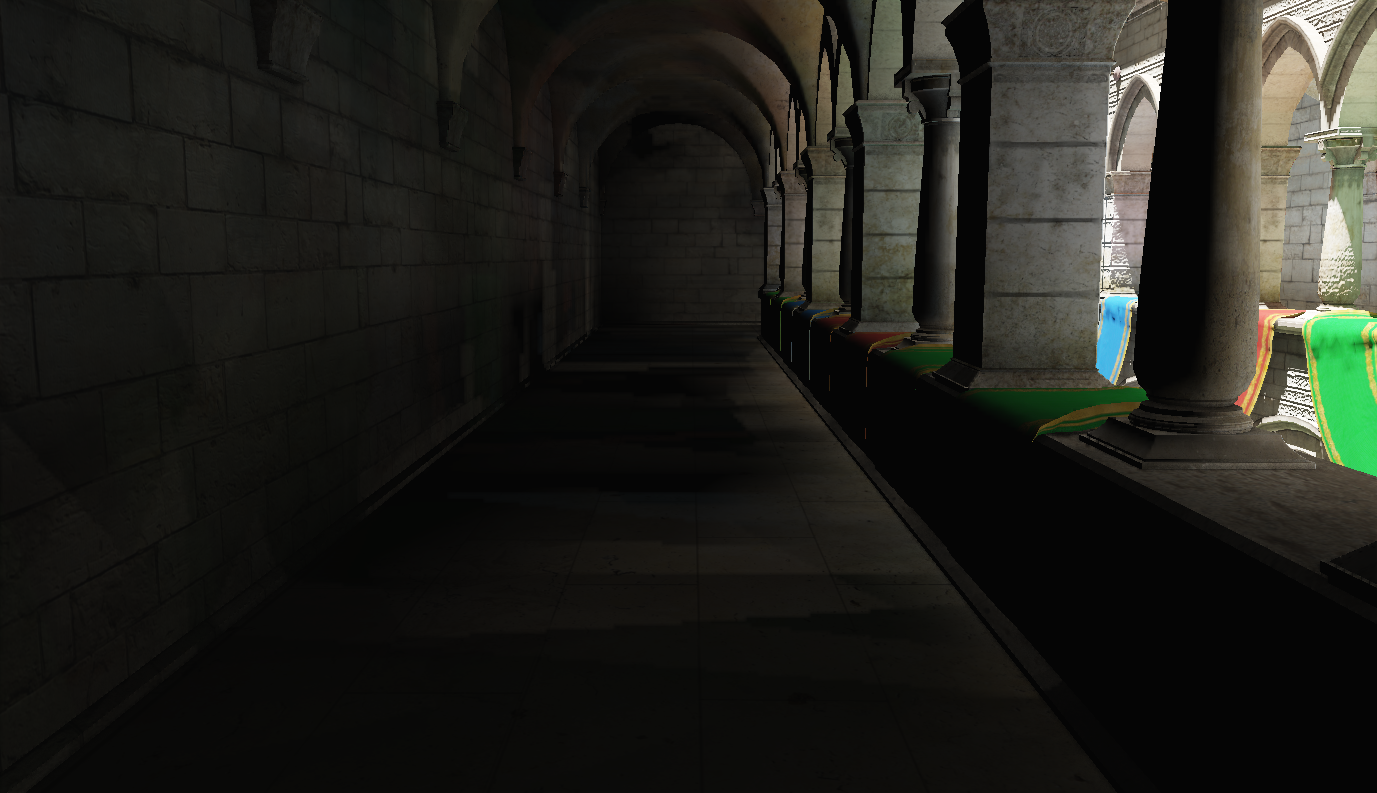
\includegraphics[width=.48\textwidth]{screenshots/bias_splat_exposure} &
      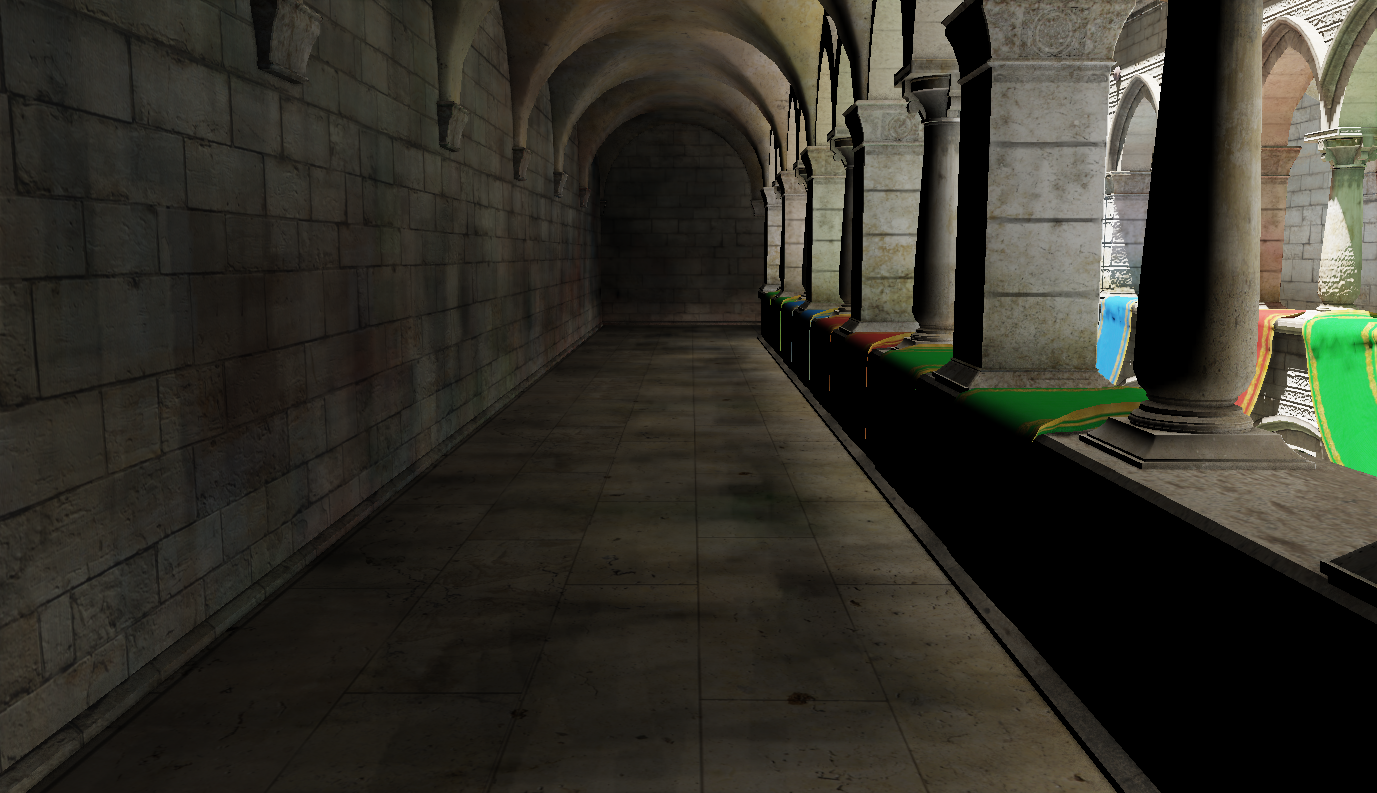
\includegraphics[width=.48\textwidth]{screenshots/bias_single_pixel_exposure}
  \end{tabular}
  \caption{Light leaks caused by using a relatively large shadow bias with the purpose to hide artifacts of the ISMs. The screenshots to the left use the splat renderer, the right ones the single-pixel renderer. Bottom row uses a higher exposure.}
  \label{fig:results:bias}
\end{figure}

Our implementation hides some of the inaccuracies of the ISMs by using a relatively large shadow bias. The resulting light leaks are shown in \Cref{fig:results:bias}. While the splat renderer fares better here, it does so mainly by darkening the whole image since it uses rather large points. The single-pixel renderer on the other hand correctly lets light shine through the columns, but shows a very noisy result on the left wall.


\todo{Screenshots when enlarging the points / making them smaller. Discuss.}

\todo{Screenshots when doing more points. either by tessellation or by collecting more. Discuss.}

\todo[color=yellow]{count point for splat renderer and output them somehow.}

\todo{Compare to max quality}

\todo[color=yellow]{implement max quality. every point into every ISM. likely render everything once for each ISM. a checkbox: when checked, compute high-quality once and do not change. back to normal when unchecked.}

\todo{for single-pixel-renderer: maybe show one full-size shadow map to show this *can* work}


\subsubsection{Performance}
\label{sec:results:ism:performance}

\begin{table}[h]
\begin{center}
    \begin{tabulary}{0.98\textwidth}{| L | L | L | L |}
        \hline
        Splat Default Settings & Single-Pixel Default Settings & Splat with Single-Pixel Settings & Single-Pixel with Splat Settings \\ \hline
        1.08\,ms & 2.74\,ms & 10.14\,ms & 2.31\,ms \\
        \hline
    \end{tabulary}
    \caption{Timings of the ISM renderers with different settings.}
    \label{tab:results:ism_timings}
\end{center}
\end{table}

\Cref{tab:results:ism_timings} shows the time needed for rendering the ISMs with both renderers and different settings.

Note that the comparison between the two renderers with default settings is not a fair one, since the single-pixel renderer uses more points and performs clamping per default. If the splat renderer is changed to behave similarly, it takes 0.3 additional milliseconds for the clamping, and 8.66 additional milliseconds for using the same technique to collect VPLs as the single-pixel renderer does. There are several reasons for this heavy slowdown: First, we implemented this by emitting multiple vertices in the geometry shader, which is known to have poor performance on current GPUs. Second, the additional fillrate and overdraw became an issue when using too many points, a bottleneck that is unlikely to occur when using the single-pixel renderer. And third, while the single-pixel renderer uses shared memory to load the 16 VPLs once, the fragment shader of the splat renderer has no access to shared memory and has to load all 16 VPLs per invocation, creating high register pressure.

Conversely, if the single-pixel renderer does not perform clamping, the push phase needs 0.07\,ms less (0.85\,ms to 0.78\,ms), and when it considers only one VPL per point, the point renderer uses 0.41\,ms less (0.65\,ms to 0.24\,ms).

Since the technique implements no adaptivity, these numbers are independent from the viewport. They are however slightly affected by VPL placement, since it influences culling. In a second scenario, where the sunlight shines directly from above, all VPLs are placed on the floor facing up. As a result, much fewer points are culled during ISM rendering, resulting in slightly higher timings. Both renderers need about 0.1\,ms more in this case.

\todo{Numbers when enlarging the points / making them smaller. Discuss. Note how the single-pixel renderer is (hopefully) not affected by point size.}

\todo{Numbers when doing more points. either by tessellation or by collecting more. Discuss.}


\subsubsection{Detailed Performance Measurements for the Single-Pixel Point Renderer}
\label{sec:results:ism:performanceSinglePixelRenderer}


\begin{table}[h]
\begin{center}
    \begin{tabulary}{0.98\textwidth}{| L | L | L | L || L |}
        \hline
        Point Collection & Point Rendering & Pull Phase & Push Phase & Total\\ \hline
        0.83\,ms & 0.65\,ms & 0.39\,ms & 0.85\,ms & 2.72\,ms\\
        \hline
    \end{tabulary}
    \caption{Timing breakdown of the single-pixel point renderer.}
    \label{tab:results:timing_breakdown_single_pixel}
\end{center}
\end{table}

\begin{table}[h]
\begin{center}
    \begin{tabulary}{0.98\textwidth}{| L | L | L | L | L | L | L | L || L | L || L |}
        \hline
        PL 1 & PL 2 & PL 3 & PL > 3 & PS > 2 & PS 2 & PS 1 & PS 0 & PL Total & PS Total & Total \\ \hline
        0.16 & 0.16 & 0.04 & 0.03   & 0.06   & 0.08 & 0.30 & 0.41 & 0.39     & 0.85     & 1.24\\
        \hline
    \end{tabulary}
    \caption{Timing breakdown of the pull (PL) and push (PS) phase. The numbers of the individual steps indicate to which mipmap level they write, which is why the pull phase starts with 1 and the push phase has descending numbers. All timings are in milliseconds.}
    \label{tab:results:timing_breakdown_pull_push}
\end{center}
\end{table}


\Cref{tab:results:timing_breakdown_single_pixel} gives more detailed performance measurements of the single-pixel renderer, while \cref{tab:results:timing_breakdown_pull_push} further breaks down the individual steps of the pull and push phase. Note how the timings scale roughly as expected (PL 3 and PS 2 are taking roughly 4 times longer than PL 2 and PS 1, respectively), but not so the first and last step. This is due to the reduced input data size (or output size, respectively), as explained in \cref{sec:impl:pullPushPostprocessing}. Also note how the push phase does take roughly the time of the pull phase if it were not for the last phase, where it writes to the full 2048\,px² of miplevel zero, whereas the first pull phase only writes to the miplevel one with 1024\,px².

\todo{Impact of packing?}

% show this is bandwidth bound. calculation how much memory is read and written, vs bandwidth of GTX 980.
%     - roughly 110MB read and written, that's 1.2ms.
%     - 16MB of that unnecessarily because of the 2nd layer of input texture
%     - By parallel reduction juju reduced by 22MB or 0.2ms.
%     - with more juju, maybe brought down to actually that time, except for the arithmetic stuff of course...


\subsubsection{Memory Usage}
\label{sec:results:ism:memory}

The point splat renderer uses no more memory than the ISM texture itself requires, which is 8\,MB for a 2048\,px² 16-bit depth buffer.

The single-pixel renderer uses additional memory. First, it uses a buffer for storing the points. This is implemented as four-channel 32-bit float texture, with the first three channels containing the position, and the last channel the radius (8 bit) and normal (24 bit, see \cite{Cigolle:2014:NormalPacking}). With a maximum point count of 2048 per ISM (keep in mind they are rendered into multiple ISMs later), this buffer uses 32\,MB.
The additional textures used are the render target of the single-pixel renderer (single-channel 2048x2048\,px, 32-bit integer, uses 16\,MB), the mipmap levels used by the pull-push algorithm (four channels, 32-bit, use approx. 22\,MB) and the final ISM (same as used by the splat renderer, uses 8MB).

Added together, the single-pixel renderer uses a total of 79\,MB, likely with room for optimization left.


\subsubsection{Problems with High Geometric Density}
\label{sec:results:ism:densityProblems}

As a more demanding test case the San Miguel scene with 7.9M triangles. The most apparent problem of the presented implementation is the lack of adaptivity to the current viewport in addition to the lack of LOD methods. As a result, all 7.9M triangles are used every frame to render the ISMs, with corresponding performance results: While the postprocessing takes the same time due to working fixed resolution textures, the point collection phase now takes 11.4\,ms, while the point rendering when using the single-pixel renderer uses an additional 5.7\,ms. The fact that the point collection phase, albeit doing no rasterization work, takes exactly the same amount of time as the splat renderer, shows how this process is bottlenecked by geometric complexity.


\begin{figure}[htb]
\centering
  \begin{tabular}{@{}c@{}}
    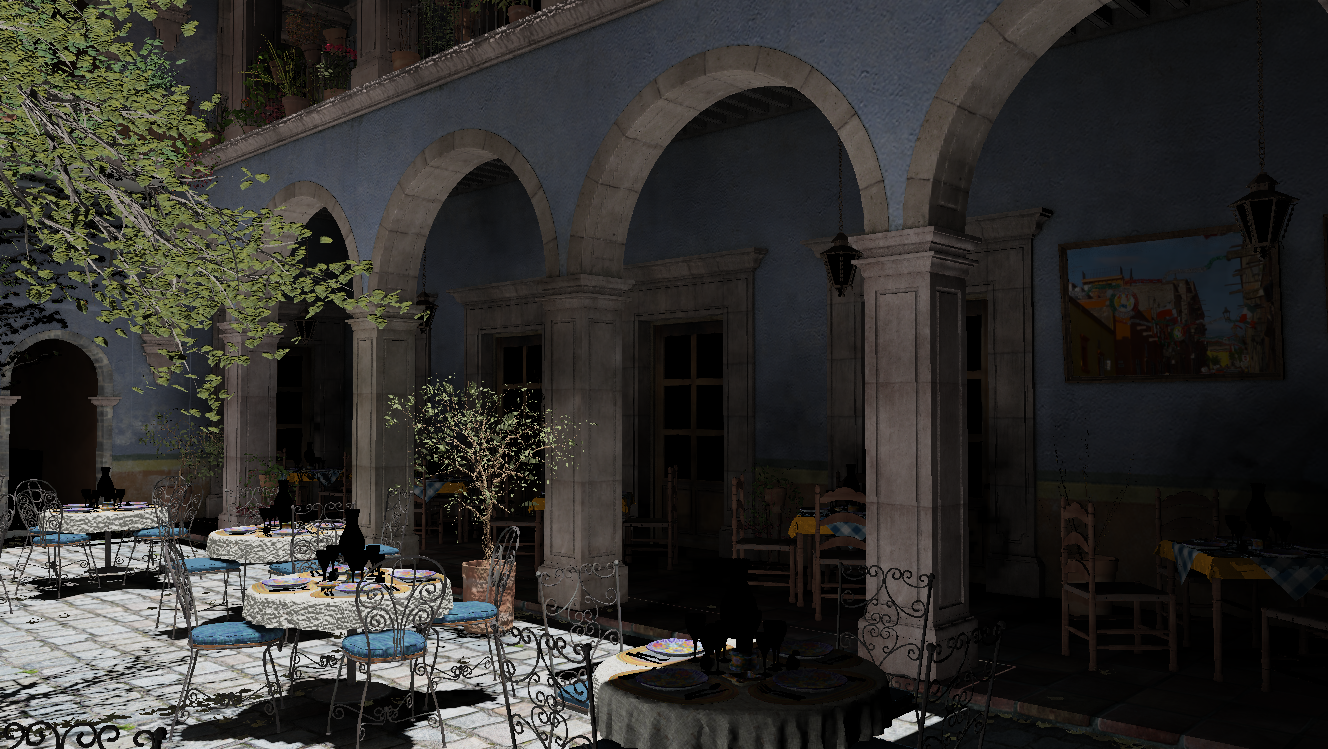
\includegraphics[width=1.0\textwidth]{screenshots/san_miguel_wide} \\
  \end{tabular}
  \caption{A rendering of the San Miguel scene in the presented implementation. Note the unnaturally dark region behind the pillars.}
  \label{fig:results:san_miguel_wide}
\end{figure}

\begin{figure}[htb]
\centering
  \begin{tabular}{@{}cc@{}}
    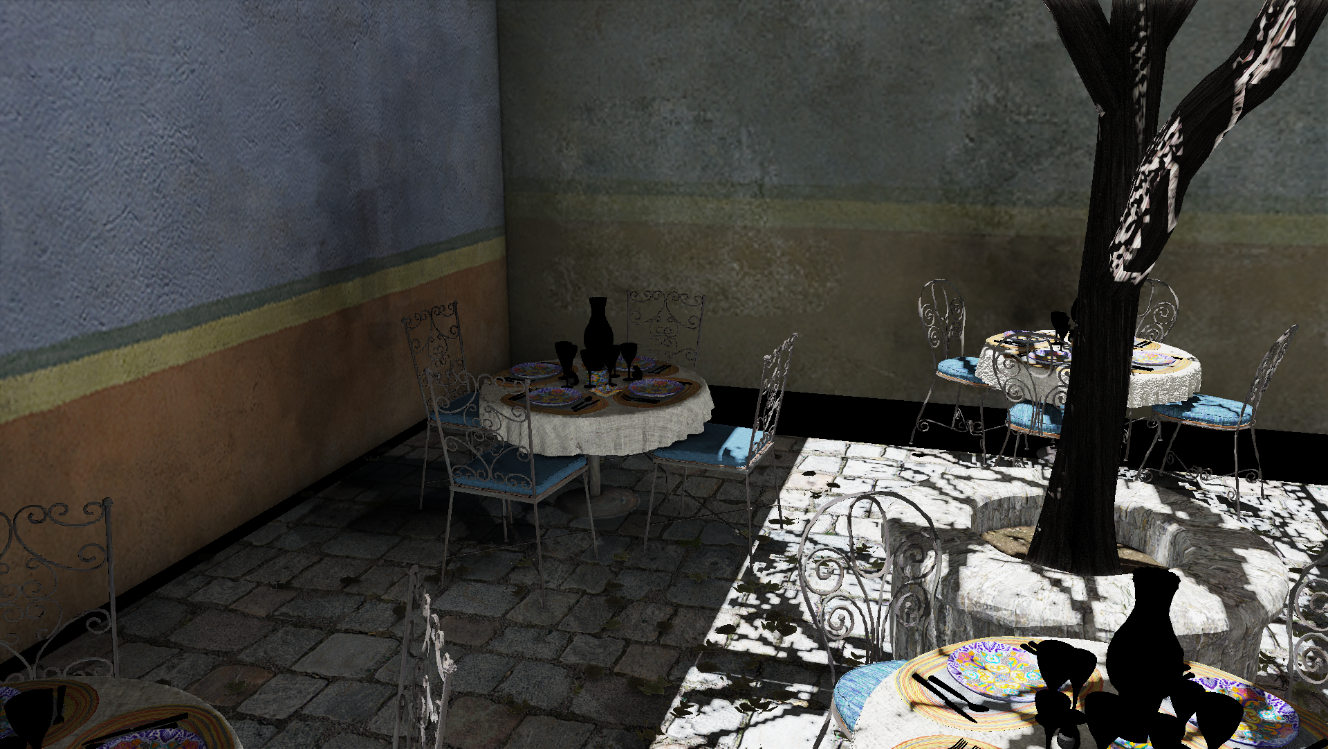
\includegraphics[width=.48\textwidth]{screenshots/san_miguel_ugly_shadow} &
    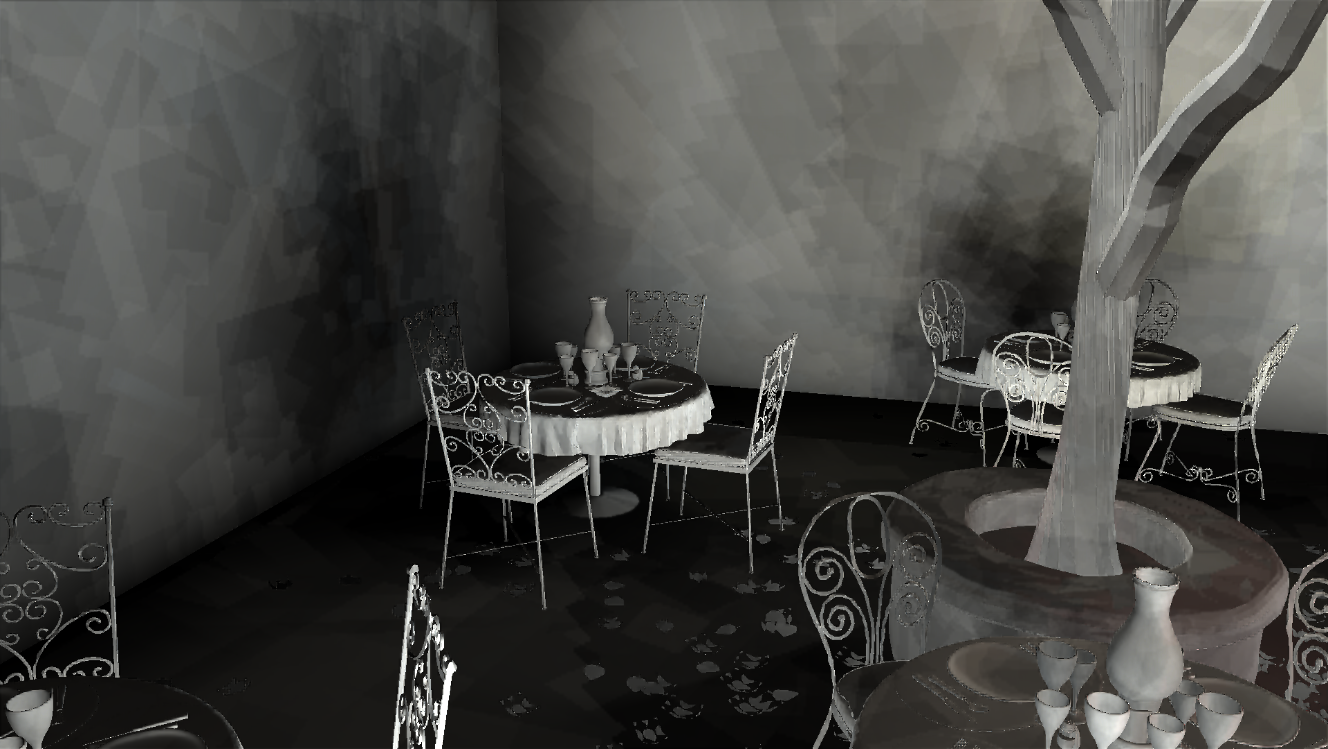
\includegraphics[width=.48\textwidth]{screenshots/san_miguel_ugly_shadow_gi_only}
  \end{tabular}
  \caption{A particularly inaccurate shadow produced by the ISMs. Right image shows only indirect light. The shadow should be much more smooth, the low-frequency noise is caused choosing random points per ISM, while the many edges of the shadows are caused by the basic shadow mapping algorithm, which performs a simple binary choice.}
  \label{fig:results:san_miguel_ugly_shadow}
\end{figure}

\Cref{fig:results:san_miguel_wide} shows an example screenshot of the San Miguel scene. There are several factors contributing to an overly dark region behind the pillars. First, during ISM rendering all points are rendered into at least one pixel, making them take out too much light if they are actually smaller than one pixel. This likely happens in case of the thin structures of the chairs. Additionally, the implementation simulates only one bounce, making it impossible for the floor behind the pillars to be lit at all.

Another problem case is shown by \Cref{fig:results:san_miguel_ugly_shadow}, where the table and chairs cast a visibly inaccurate shadow.


\subsection{Comparison of the Splat and Single-Pixel Renderer}
\label{sec:results:ism:comparison}

The single-pixel renderer provides numerous advantages over the splat renderer: Using a compute shader to render the points lifts the restrictions of the fixed-function pipeline and e.\,g., enables rendering each point into multiple ISMs without large performance losses. Quality-wise, it can reproduce surfaces more accurately by correctly interpolating between points.

The drawbacks obviously include the additional rendering time and memory. Besides, the added complexity should not be underestimated. Specifically, we found it hard to fine-tune the pull-push algorithm to give us satisfactory results, especially in the face of the low resolutions of ISMs and the limited data available for reconstruction after selecting a random and sparse set of points.

\todo{Add notes about scaling when i have point counts}



\subsection{Discussion}
\label{sec:results:ism:discussion}

Imperfect shadow maps have several deficits, some of which are inherent to the technique and difficult to solve, others are specific to the implementation choices and tradeoffs in our implementation and might be easier to overcome.

First, ISMs reduce the scene's geometry to points. At the resolution that is achievable in a real-time budget, this is already a rough approximation that loses a lot of accuracy.

Second, because a sparse set of points is used for each ISM, each point must be enlarged to accommodate for the neighboring points that are likely missing in the chosen ISM. For instance, if an area is represented by a thousand points and only one tenth of all points is used for each ISM, each remaining point's area must be enlarged by a factor of ten to result in an equally large area in the rendered output. Of course, this approach leads to deformed geometry since points at the edges of the area get enlarged as well, growing over the borders of the original geometry.

Third, there are also numerical issues. For instance, both the splatting and postprocessing approaches ignore the distortion caused by the projection, and thus might render even simple surfaces incorrectly. This contributes to the necessity of using a relatively large shadow bias. This can likely be solved, albeit at the cost of additional complexity.

Fourth, and this is in our view the most important shortcoming, ISMs handle geometry in the vicinity to VPLs badly as can be seen in \cref{fig:results:leaks}. To sufficiently approximate such surfaces when rendering ISMs, one would need to greatly increase the number of points created near VPLs, possibly in addition to stepping away from using a fully random approach for point selection and select a specific point set for each ISM depending on the VPLs location.

As for most global illumination algorithms, a massive improvement would be to differentiate between large-scale scene geometry that is important for diffuse light bounces, and smaller geometry of lesser importance. While the latter can possibly be ignored altogether with only minor losses in quality, the shape of large-scale geometry is all the more important to preserve (relatively) precisely.

The San Miguel scene is a good example for this: While the small detail work like dishes and small plants make up most of the geometry and thus most of the rendering time, they contribute only very little to global illumination. This is where our implementation suffers most from the lack of level-of-detail methods.


\todo[color=yellow]{implement some moving object. show temporal coherency when it moves. or even moving spherical light.}


\section{Interleaved Shading with Compute Shaders}
\label{sec:results:interleavedShading}

Interleaved shading substantially reduces the number of lights that are processed per pixel. Using a 4x4 interleaving pattern, each pixel processes only a sixteenth of all lights, ideally speeding up the final gathering phase by a factor of 16. However, an additional blur pass is required to mask the noise that results from interleaving, which takes additional time.


\begin{table}[h]
    \begin{center}
        \begin{tabulary}{0.98\textwidth}{| L | L | L | L | L |}
            \hline
            Without IS & With IS & Speedup & Blur Pass & Speedup with blur\\ \hline
            40.24\,ms & 2.61\,ms & 15.42 & 0.63\,ms & 12.42\\
            \hline
        \end{tabulary}
        \caption{Timings of interleaved shading (IS) with a block size of 4x4. Note that the blur pass is mandatory when using interleaved shading, the middle column merely illustrates the efficiency of the presented implementation, while the last column shows the practical speedup that is achieved.}
        \label{tab:results:timings_interleaved_shading}
    \end{center}
\end{table}



\begin{figure}[htb]
    \centering
    \begin{subfigure}[b]{0.20\textwidth}
        \centering
        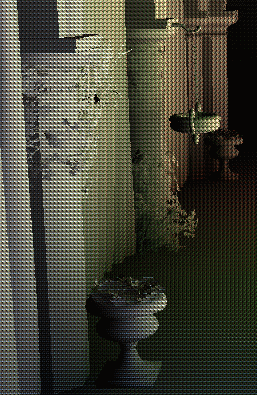
\includegraphics[width=.95\textwidth]{screenshots/interleaved_before}
        \caption{}
        \label{fig:results:interleaved_before}
    \end{subfigure}%
    \begin{subfigure}[b]{0.20\textwidth}
        \centering
        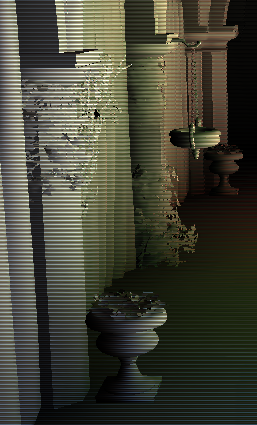
\includegraphics[width=.95\textwidth]{screenshots/interleaved_horizontal_blur}
        \caption{}
        \label{fig:results:interleaved_horizontal_blur}
    \end{subfigure}%
    \begin{subfigure}[b]{0.20\textwidth}
        \centering
        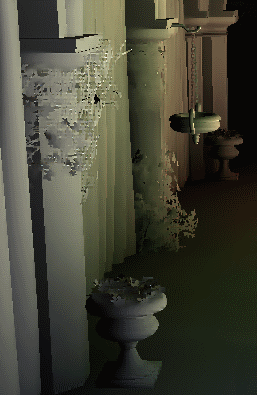
\includegraphics[width=.95\textwidth]{screenshots/interleaved_final}
        \caption{}
        \label{fig:results:interleaved_final}
    \end{subfigure}%
    \begin{subfigure}[b]{0.20\textwidth}
        \centering
        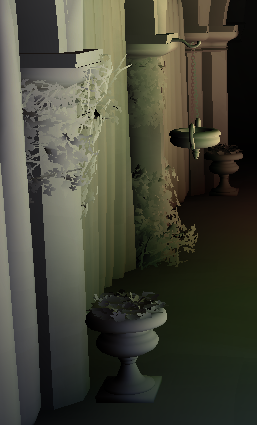
\includegraphics[width=.95\textwidth]{screenshots/interleaved_without}
        \caption{}
        \label{fig:results:interleaved_without}
    \end{subfigure}%
    \begin{subfigure}[b]{0.20\textwidth}
        \centering
        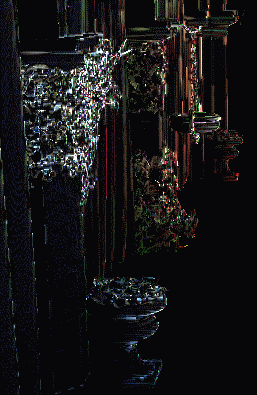
\includegraphics[width=.95\textwidth]{screenshots/interleaved_difference_gi}
        \caption{}
        \label{fig:results:interleaved_difference_gi}
    \end{subfigure}
    \begin{subfigure}[b]{0.32\textwidth}
        \centering
        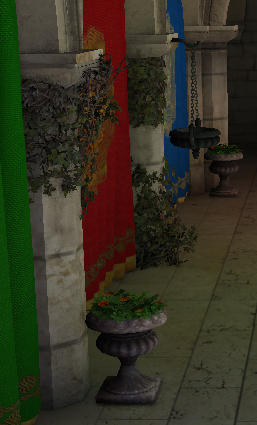
\includegraphics[width=.95\textwidth]{screenshots/interleaved_without_textured}
        \caption{}
        \label{fig:results:interleaved_without_textured}
    \end{subfigure}
    \begin{subfigure}[b]{0.32\textwidth}
        \centering
        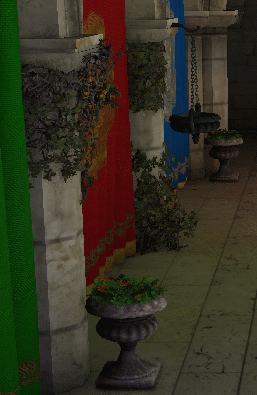
\includegraphics[width=.95\textwidth]{screenshots/interleaved_with_textured}
        \caption{}
        \label{fig:results:interleaved_with_textured}
    \end{subfigure}
    \begin{subfigure}[b]{0.32\textwidth}
        \centering
        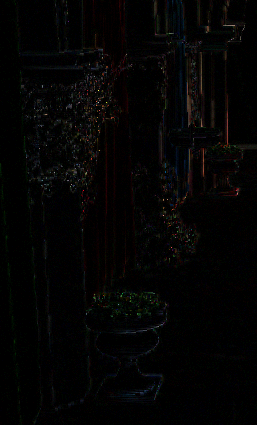
\includegraphics[width=.95\textwidth]{screenshots/interleaved_difference_shaded}
        \caption{}
        \label{fig:results:interleaved_difference_shaded}
    \end{subfigure}

      \caption{Interleaved shading results. Top row shows indirect light only. From left to right: (a) Result of the final gathering phase without the geometry-aware blur, (b) with the horizontal phase of the blur applied, (c) with both phases applied, (d) result of the final gathering phase without using interleaved shading, (e) difference between the (c) and (d). Bottom row: (f) final result after blending when using interleaved shading, (g) whithout interleaved shading, (h) difference between (f) and (g). Difference values are multiplied by four.}
      \label{fig:results:interleaved_quality}
\end{figure}


\Cref{tab:results:timings_interleaved_shading} shows timings of the presented implementation. Most notably, the interleaved shading technique introduces very little overhead, as indicated by the speedup of 15.42 compared to the theoretical maximum of 16. In absolute terms, a speedup of 16 would require the final gathering phase to take 2.51\,ms. As a result, the technique introduces 0.1\,ms of overhead.

When considering the blur phase, the overhead adds up to 0.73\,ms and the speedup is lowered to 12.42. Of course this is still a substantial improvement, especially considering the negligible quality impact.

This technique uses an additional buffer for storing the intermediate result of the blur phase, while the final result can be written into the same texture that was used for final gathering. The texture format \texttt{GL\_R11F\_G11F\_B10F} is used here, resulting in roughly 2\,MB additional storage at full HD. The presented implementation does not re-use the final gathering texture to keep the results of all stages available for debugging purposes.


\subsubsection{Discussion}
Interleaved shading is an obvious win for many-light global illumination methods. Paying the full cost of evaluating all VPLs per shading point is simply unnecessary due to the low-frequency nature of global illumination. Adapting the shading frequency to a similarly low level is the only reasonable choice for real-time applications.

In fact, given the unnoticable quality impact (\Cref{fig:results:interleaved_quality}) of interleaved shading when using a 4x4 block size, larger block sizes, e.\,g., 8x8 as used by \citet{hedman2016sequential} should be considered. Especially with the advent of high-resolution displays, lowering the shading frequency of global illumination effect even further might be necessary to keep the costs down to a reasonable level. However, the performance gains from lower sample counts will be offset in part by larger blur radii that come with larger block sizes.

Going further, this technique is limited by how well the blur phase will be able to mask the noise in more difficult areas with lots of depth discontinuities like vegetation. It seems imaginable to extend interleaved shading with ???, which collect fragments that receive too few information during shading and blurring with the purpose to perform a second pass on those fragments, enhancing the problematic areas. Temporal reprojection methods that re-use information from previous frames and use different sets of VPLs per frame would be another natural extension of interleaved shading.

\todo{that fragment collecting reference}

\todo{put VPL shuffling comparison anywhere}



\section{Clustered Deferred Shading}
\label{sec:results:clusteredShading}

Clustered Deferred Shading and Tiled Deferred Shading reduce the number of light calculation operations by clustering fragments and culling lights against those clusters. As such, if implemented correctly, they do not affect quality at all, but are purely performance optimizations.

\begin{table}[h]
    \begin{center}
        \begin{tabulary}{0.98\textwidth}{| L | L | L | L | L |}
            \hline
            Scene & Without CS/TS & With CS & With TS \\ \hline
            Sponza 1 & 3.41\,ms & 2.80\,ms & 2.40\\
            Sponza 2 & 3.94\,ms & 3.63\,ms & 3.09\\
            Sponza 3 & 2.68\,ms & 1.64\,ms & 1.34\\
            San Miguel & 4.75\,ms & 5.21\,ms & 4.43\\
            \hline
        \end{tabulary}
        \caption{Timings of the final gathering stage without optimizations, with clustered shading (CS) and with tiled shading (TS). Each line is a different camera position. Note that the timing ``With CS'' includes roughly 0.06\,ms for the clustering phase and 0.13\,ms for the light list phase.}
        \label{tab:results:timings_clustered_shading}
    \end{center}
\end{table}

As visible in \Cref{tab:results:timings_clustered_shading}, both clustered shading and tiled deferred shading can improve the performance of the final gathering phase considerably, in one of the measurements 50\,\% of the computation time is saved with tiled shading.


clustered shading advantage is primarily depth discontinuities

What is interesting though is that clustered shading, being the successor of tiled shading, performs noticeably worse in the context of many-light methods. This is true even for the San Miguel scene, in which the higher amount of depth discontinuities should be favorable to clustered shading. While these performance characteristics might be specific to the presented implementation, there are plausible reasons that they might apply generally. Due to the infinite light radii used, the percentage of culled lights is generally low. Therefore it might be the better choice to optimize for the worst case and implement a low overhead solution like tiled shading, instead of a more accurate solution like clustered shading that might improve the culling rate, but comes with more overhead.

An impression of the amount of overhead introduced by clustered shading is given by the San Miguel scene, from which the last line of measurements is taken. This scene runs much slower even when only considering the final gathering phase, because most VPLs are placed on the walls and floor, pointing inwards or upwards respectively. Therefore much of the geometry lies on the illuminated side of most VPLs, resulting in very little performance gains from culling.

With a low culling rate, clustered shading actually slows down the final gathering phase by 0.46\,ms. While 0.19\,ms of these are fixed costs added by the clustering and light list calculation phases, the final gathering shader itself got 0.27\,ms slower as well. This might be caused by the indirection when accessing lights, since instead of reading from the light buffer directly, the light list with indices is accessed first before reading the light buffer with a dynamic index. Another explanation might be the divergent data flow, since threads from the same work group can access different light lists and thus different light data and shadow maps, possibly hurting cache efficiency.

As discussed in section \Cref{sec:impl:clusteredShading}, clustered shading consumes about 2\,MB of memory. The tiled shading algorithm however, being integrated into the final gathering shader, uses no additional VRAM at all.

The presented measurements make tiled shading seem like a clear winner, but as so often the situation is more complicated. The integration of tiled shading into the final gathering shader, while an efficient and easy to implement solution, is inherently less flexible than clustered shading. For instance, \citet{olsson2012clustered} propose to use normals as another dimension besides the three spatial ones, further improving culling efficiency. While this is likely easy to integrate into the more flexible approach taken with clustered shading, the integrated tiled shading is constrained by the amount of available shared memory, which makes it challenging to take additional dimensions into account.

%!TEX root = foo-thesis.tex


\chapter{Conclusion}
\label{chap:conclusion}

\todo[color=blue]{Conclusion}


\chapter{Todos}

\subsubsection{figures}

\todo[inline]{make figures nicer}

\todo[inline]{implementation pipeline \ref{fig:RenderingPipelineOverview} adds little value over concept pipeline.}

\todo[inline]{nicer \Cref{fig:results:RSMBuffers}, maybe only one large divided in thirds, or zoomins}

\todo[inline]{Pipeline figures for all sections in implementation. e.g. create RSM, which is then sampled, and the samples are put into two buffers.}

\todo[inline]{Interleaved shading algorithm figure comparing buffer splitting vs compute shaders in addition to pipeline figure \Cref{sec:impl:interleavedShading}}

\todo[inline]{Temporal coherence/frame-to-frame diff when light moves figure. end of \Cref{sec:results:RsmAndVplSampling}}

\todo[inline]{more debug views, debug data visualizations}
\todo[inline]{daniel's pipeline visualizations, see emails}


\subsubsection{content}

\todo[inline]{nicer, less structure-in-your-face introduction in \Cref{sec:intro:gi:components}, in order to ... it is necessary to have an understanding of...}

\todo[inline]{more conclusion by adding summaries of the approaches, how did we come to these conclusions, we've been able to show...}

\todo[inline]{abstract and zusammenfassung}

\todo[inline]{Lui: summaries at the end of chapters}

\todo[inline]{Lui: replace "this chapter will ..." by introductory sentences from first section}

\todo[inline]{Lui: more references on first few pages}

\todo[inline]{some closing remarks. add some personal evaluations, broad statement about complexity}

\todo[inline]{summarize ISM deficits in ISM discussion \Cref{sec:results:ism:discussion}}

\todo[inline]{do some pseudocode}

\todo[inline]{put VPL shuffling comparison anywhere, maybe results \Cref{sec:results:ism:quality}}

\todo[inline]{4k tests}

\todo[inline]{ISM quality: for single-pixel-renderer: maybe show one full-size shadow map to show this *can* work. \Cref{sec:results:ism:quality}}

\todo[inline,color=yellow]{ISMs: point count for splat renderer and output them somehow. \Cref{sec:results:ism:quality}}

\todo[inline]{ISM comparison: Add notes about scaling when i have point counts \Cref{sec:results:ism:comparison}}

\todo[inline]{ISM performance: Numbers when enlarging the points / making them smaller. Discuss. Note how the single-pixel renderer is (hopefully) not affected by point size. \Cref{sec:results:ism:quality}}

\todo[inline]{ISM quality / performance: Screenshots and performance numbers when doing more points. either by tessellation or by collecting more. Discuss. \Cref{sec:results:ism:quality}}



\subsubsection{code}

\todo[inline,color=yellow]{implement some moving object. show temporal coherency when it moves. or even moving spherical light. \Cref{sec:results:ism}}

\todo[inline,color=yellow]{rename gi shader to final gathering. other renames?}

\todo[inline,color=yellow]{investigate into interleaving via shared memory in 2x2 groups (that is, one work group reads 2x2 interleaved pixels instead of one)}

\todo[inline,color=yellow]{implement ISM max quality. every point into every ISM. likely render everything once for each ISM. a checkbox: when checked, compute high-quality once and do not change. back to normal when unchecked. \Cref{sec:results:ism:quality}}

\todo[inline,color=yellow]{ISM performance: Impact of packing? \Cref{sec:results:ism:performanceSinglePixelRenderer}}


\subsubsection{misc}

\todo[inline]{cleanup repository. rebase and cut the first unrelated commits out? decide on repository name, and maybe github name.}


\todo[inline]{brighter version for print}
\todo[inline]{noindent after figures}
\todo[inline]{latex warnings}
\todo[inline]{esp. overflows}
\todo[inline]{orphans and widows, also single words on a line}
\todo[inline]{spell checking}


% %!TEX root = foo-thesis.tex

\chapter{Examples}

At vero eos et accusam et justo duo dolores et ea rebum. Stet clita kasd gubergren, no sea takimata sanctus est Lorem ipsum dolor sit amet. Lorem ipsum dolor sit amet, consetetur sadipscing elitr, sed diam nonumy eirmod tempor invidunt ut labore et \citep{Aubert.Kornprobst-2006} dolore magna aliquyam erat, sed diam voluptua. At vero eos et accusam et justo duo dolores et ea rebum. Stet clita kasd gubergren, no sea takimata sanctus est Lorem ipsum dolor sit amet.


\subsection{Stet clita kasd gubergren}
Consetetur \citep{Goshtasby.Satter-2008} sadipscing elitr, sed diam nonumy eirmod tempor invidunt ut labore et dolore magna aliquyam erat, sed diam voluptua. At vero eos et accusam et justo duo dolores et ea rebum. Stet clita kasd gubergren, no sea takimata sanctus est Lorem ipsum dolor sit amet. Lorem ipsum dolor sit amet, consetetur sadipscing elitr, sed diam nonumy eirmod tempor invidunt ut labore et dolore magna aliquyam erat, sed diam voluptua. At vero eos et accusam et justo duo dolores et ea rebum. Stet clita kasd gubergren, no sea takimata sanctus est Lorem ipsum dolor sit amet. Lorem ipsum dolor sit amet, consetetur sadipscing elitr, sed diam nonumy eirmod tempor invidunt ut labore et dolore magna aliquyam erat, sed diam voluptua. At vero eos et accusam et justo duo dolores et ea rebum. Stet clita kasd gubergren, no sea takimata sanctus.
\begin{itemize}
\item Duis autem vel eum iriure dolor in hendrerit in vulputate velit esse molestie consequat, vel illum dolore eu feugiat nulla facilisis at vero eros et
\item Et iusto odio dignissim qui blandit praesent luptatum zzril delenit augue duis dolore te feugait nulla facilisi. Lorem ipsum dolor sit.
\begin{itemize}
\item Duis autem vel eum iriure dolor in hendrerit in vulputate velit esse molestie consequat, vel illum dolore eu feugiat nulla facilisis at vero eros et.
\item Et iusto odio dignissim qui blandit praesent luptatum zzril delenit augue duis dolore te feugait nulla facilisi. Lorem ipsum dolor sit.
\item Amet, consectetuer adipiscing elit, sed diam nonummy nibh euismod tincidunt ut laoreet dolore magna aliquam erat volutpat.
\end{itemize}
\item Amet, consectetuer adipiscing elit, sed diam nonummy nibh euismod tincidunt ut laoreet dolore magna aliquam erat volutpat.
\end{itemize}
Duis autem vel eum iriure dolor in hendrerit in vulputate velit esse molestie consequat, vel illum dolore eu feugiat nulla facilisis at vero eros et accumsan et iusto odio dignissim qui blandit praesent luptatum zzril delenit augue duis dolore te feugait nulla facilisi. Lorem ipsum dolor sit amet, consectetuer adipiscing elit, sed diam nonummy nibh euismod tincidunt ut laoreet dolore magna aliquam erat volutpat.
Ut wisi enim ad minim veniam, quis nostrud exerci tation ullamcorper suscipit lobortis nisl ut aliquip ex ea commodo consequat. Duis autem vel eum iriure dolor in hendrerit in vulputate velit esse molestie consequat, vel illum dolore eu feugiat nulla facilisis at vero eros et accumsan et iusto odio dignissim qui blandit praesent luptatum zzril delenit augue duis dolore te feugait nulla facilisi.

\subsection{Stet clita kasd gubergren}
Nam liber tempor cum soluta nobis eleifend option congue nihil imperdiet doming id quod mazim placerat facer possim assum. Lorem ipsum dolor sit amet, consectetuer adipiscing elit, sed diam nonummy nibh euismod tincidunt ut laoreet dolore magna aliquam erat volutpat. Ut wisi enim ad minim veniam, quis nostrud exerci tation ullamcorper suscipit lobortis nisl ut aliquip ex ea commodo consequat.
Duis autem vel eum iriure dolor in hendrerit in vulputate velit esse molestie consequat, vel illum dolore eu feugiat nulla facilisis.
At vero eos et accusam et justo duo dolores et ea rebum. Stet clita kasd gubergren, no sea takimata sanctus est Lorem ipsum dolor sit amet. Lorem ipsum dolor sit amet, consetetur sadipscing elitr, sed diam nonumy eirmod tempor invidunt ut labore et dolore magna aliquyam erat, sed diam voluptua. At vero eos et accusam et justo duo dolores et ea rebum. Stet clita kasd gubergren, no sea takimata sanctus est Lorem ipsum dolor sit amet. Lorem ipsum dolor sit amet, consetetur sadipscing elitr, At accusam aliquyam diam diam dolore dolores duo eirmod eos erat, et nonumy sed tempor et et invidunt justo labore Stet clita ea et gubergren, kasd magna no rebum. sanctus sea sed takimata ut vero voluptua. est Lorem ipsum dolor sit amet. Lorem ipsum dolor sit amet, consetetur sadipscing elitr, sed diam nonumy eirmod tempor invidunt ut labore et dolore magna aliquyam erat.

\begin{figure}
    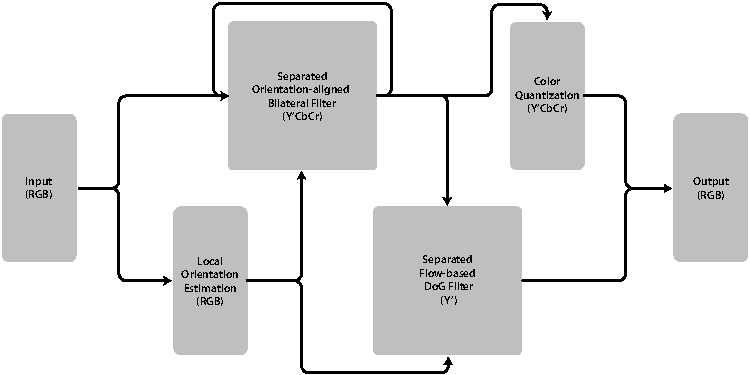
\includegraphics[width=\textwidth]{graphics/test3}
    \caption{Stet clita kasd gubergren, no sea takimata sanctus est Lorem ipsum dolor sit amet. Lorem ipsum dolor sit amet, consetetur sadipscing elitr.}
\end{figure}

Consetetur sadipscing elitr, \citep{Yang.etal-1996} sed diam nonumy eirmod tempor invidunt ut labore et dolore magna aliquyam erat, sed diam voluptua. At vero eos et accusam et justo duo dolores et ea rebum. Stet clita kasd gubergren, no sea takimata sanctus est Lorem ipsum dolor sit amet. Lorem ipsum dolor sit amet, consetetur sadipscing elitr, sed diam nonumy eirmod tempor invidunt ut labore et dolore magna aliquyam erat, sed diam voluptua. At vero eos et accusam et justo duo dolores et ea rebum. Stet clita kasd gubergren, no sea takimata sanctus est Lorem ipsum dolor sit amet. Lorem ipsum dolor sit amet, consetetur sadipscing elitr, sed diam nonumy eirmod tempor invidunt ut labore et dolore magna aliquyam erat, sed diam voluptua. At vero eos et accusam et justo duo dolores et ea rebum. Stet clita kasd gubergren, no sea takimata sanctus.


\subsection{At vero eos et accusam}
Ut wisi enim ad minim veniam, quis nostrud exerci tation ullamcorper suscipit lobortis nisl ut aliquip ex ea commodo consequat. Duis autem vel eum iriure dolor in hendrerit in vulputate velit esse molestie consequat, vel illum dolore eu feugiat \citep{Guichard.Morel-2003} nulla facilisis at vero eros et accumsan et iusto odio dignissim qui blandit praesent luptatum zzril delenit augue duis dolore te feugait nulla facilisi.
Nam liber tempor cum soluta nobis eleifend option congue nihil imperdiet doming id quod mazim placerat facer possim assum. Lorem ipsum dolor sit amet, consectetuer adipiscing elit, sed diam nonummy nibh euismod tincidunt ut laoreet dolore magna aliquam erat volutpat. Ut wisi enim ad minim veniam, quis nostrud exerci tation ullamcorper suscipit lobortis nisl ut aliquip ex ea commodo consequat.
Duis autem vel eum iriure dolor in hendrerit in vulputate velit esse molestie consequat, vel illum dolore eu feugiat nulla facilisis.

\begin{figure}
    \centering%
    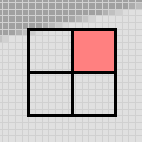
\includegraphics[width=0.32\textwidth]{graphics/test0}
    \caption{Stet clita kasd gubergren, no sea takimata sanctus est.}
\end{figure}


\section{At accusam aliquyam}
At vero eos et accusam et justo duo dolores et ea rebum. Stet clita kasd gubergren, no sea takimata sanctus est Lorem ipsum dolor sit amet. Lorem ipsum dolor sit amet, consetetur sadipscing elitr, sed diam nonumy eirmod tempor invidunt ut labore et dolore magna aliquyam erat, sed diam voluptua. At vero eos et accusam et justo duo dolores et ea rebum. Stet clita kasd gubergren, no sea takimata sanctus est Lorem ipsum dolor sit amet. Lorem ipsum dolor sit amet, consetetur sadipscing elitr, At accusam aliquyam diam diam dolore dolores duo eirmod eos erat, et nonumy sed tempor et et invidunt justo labore Stet clita ea et gubergren, kasd magna no rebum. sanctus sea sed takimata ut vero voluptua. est Lorem ipsum dolor sit amet. Lorem ipsum dolor sit amet, consetetur sadipscing elitr, sed diam nonumy eirmod tempor invidunt ut labore et dolore magna aliquyam erat.
\begin{itemize}
\item Duis autem vel eum iriure dolor in hendrerit in vulputate velit esse molestie consequat, vel illum dolore eu feugiat nulla facilisis at vero eros et
\item Et iusto odio dignissim qui blandit praesent luptatum zzril delenit augue duis dolore te feugait nulla facilisi. Lorem ipsum dolor sit.
\item Amet, consectetuer adipiscing elit, sed diam nonummy nibh euismod tincidunt ut laoreet dolore magna aliquam erat volutpat.
\end{itemize}


Duis autem vel eum iriure dolor in hendrerit in vulputate velit esse molestie consequat, vel illum dolore eu feugiat nulla facilisis at vero eros et accumsan et iusto odio dignissim qui blandit praesent luptatum zzril delenit augue duis dolore te feugait nulla facilisi. Lorem ipsum dolor sit amet, consectetuer adipiscing elit, sed diam nonummy nibh euismod tincidunt ut laoreet dolore magna aliquam erat volutpat.

\begin{figure}
    \subcaptionbox{\label{fig:test3a}Test 1}{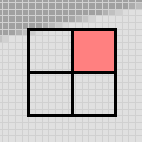
\includegraphics[width=0.32\textwidth]{graphics/test0}}%
    \hfill%
    \subcaptionbox{\label{fig:test3b}Test 2}{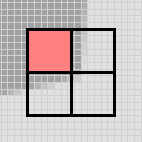
\includegraphics[width=0.32\textwidth]{graphics/test1}}%
    \hfill%
    \subcaptionbox{\label{fig:test3c}Test 3}{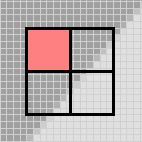
\includegraphics[width=0.32\textwidth]{graphics/test2}}%
    \caption{Stet clita kasd gubergren, no sea takimata}
    \label{fig:test3}
\end{figure}

\textbf{Ut wisi enim} ad minim veniam, quis nostrud exerci tation ullamcorper suscipit lobortis nisl ut aliquip ex ea commodo consequat. Duis autem vel eum iriure dolor in hendrerit in vulputate velit esse molestie consequat, vel illum dolore eu feugiat nulla facilisis at vero eros et accumsan et iusto odio dignissim qui blandit praesent luptatum zzril delenit augue duis dolore te feugait nulla facilisi.
Nam liber tempor cum soluta nobis eleifend option congue nihil imperdiet doming id quod mazim placerat facer possim assum. Lorem ipsum dolor sit amet, consectetuer adipiscing elit, sed diam nonummy nibh euismod tincidunt ut laoreet dolore magna aliquam erat volutpat. Ut wisi enim ad minim veniam, quis nostrud exerci tation ullamcorper suscipit lobortis nisl ut aliquip ex ea commodo consequat.
Duis autem vel eum iriure dolor in hendrerit in vulputate velit esse molestie consequat, vel illum dolore eu feugiat nulla facilisis.



\lstinputlisting[float,caption={Consetetur sadipscing elitr, sed diam nonumy eirmod tempor invidunt ut labore et dolore magna.}]{graphics/bf.glsl}%

At vero eos et accusam et justo duo dolores et ea rebum. Stet clita kasd gubergren, no sea takimata sanctus est Lorem ipsum dolor sit amet. Lorem ipsum dolor sit amet, consetetur sadipscing elitr, sed diam nonumy eirmod tempor invidunt ut labore et dolore magna aliquyam erat, sed diam voluptua. At vero eos et accusam et justo duo dolores et ea rebum. Stet clita kasd gubergren, no sea takimata sanctus est Lorem ipsum dolor sit amet. Lorem ipsum dolor sit amet, consetetur sadipscing elitr, At accusam aliquyam diam diam dolore dolores duo eirmod eos erat, et nonumy sed tempor et et invidunt justo labore Stet clita ea et gubergren, kasd magna no rebum. sanctus sea sed takimata ut vero voluptua. est Lorem ipsum dolor sit amet. Lorem ipsum dolor sit amet, consetetur sadipscing elitr, sed diam nonumy eirmod tempor invidunt ut labore et dolore magna aliquyam erat.

\begin{figure}
    \subcaptionbox{Test 1}{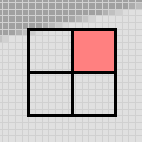
\includegraphics[width=0.32\textwidth]{graphics/test0}}%
    \hfill%
    \subcaptionbox{Test 2}{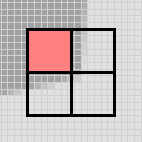
\includegraphics[width=0.32\textwidth]{graphics/test1}}%
    \hfill%
    \subcaptionbox{Test 3}{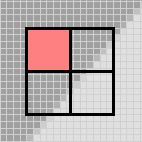
\includegraphics[width=0.32\textwidth]{graphics/test2}}%
    \par\medskip%
    \subcaptionbox{Test 1}{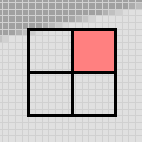
\includegraphics[width=0.32\textwidth]{graphics/test0}}%
    \hfill%
    \subcaptionbox{Test 2}{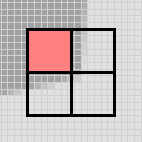
\includegraphics[width=0.32\textwidth]{graphics/test1}}%
    \hfill%
    \subcaptionbox{Test 3}{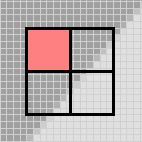
\includegraphics[width=0.32\textwidth]{graphics/test2}}%
    \caption{Stet clita kasd gubergren, no sea takimata sanctus est. Stet clita kasd gubergren, no sea takimata sanctus est.}
\end{figure}

Ut wisi enim ad minim veniam, quis nostrud exerci tation ullamcorper suscipit lobortis nisl ut aliquip ex ea commodo consequat. Duis autem vel eum iriure dolor in hendrerit in vulputate velit esse molestie consequat, vel illum dolore eu feugiat nulla facilisis at vero eros et accumsan et iusto odio dignissim qui blandit praesent luptatum zzril delenit augue duis dolore te feugait nulla facilisi.
Nam liber tempor cum soluta nobis eleifend option congue nihil imperdiet doming id quod mazim placerat facer possim assum. Lorem ipsum dolor sit amet, consectetuer adipiscing elit, sed diam nonummy nibh euismod tincidunt ut laoreet dolore magna aliquam erat volutpat. Ut wisi enim ad minim veniam, quis nostrud exerci tation ullamcorper suscipit lobortis nisl ut aliquip ex ea commodo consequat.
Duis autem vel eum iriure dolor in hendrerit in vulputate velit esse molestie consequat, vel illum dolore eu feugiat nulla facilisis.

% %!TEX root = foo-thesis.tex

\chapter{Sample File from SIAM \LaTeX\ Book Macro Package}

%\begin{chapterquote}[120pt]
%We have nothing to fear but fear itself.\\
%---{\upshape Franklin D. Roosevelt}\\[6pt]
%I am not a crook.\\
%---{\upshape Richard M. Nixon}
%\end{chapterquote}

\newtheorem{theorem}{Theorem}
\newtheorem{lemma}{Lemma}
\newtheorem{proposition}{Proposition}
\newtheorem{corollary}{Corollary}
\newtheorem{definition}{Definition}

\newcommand{\pe}{\psi}
\def\d{\delta}
\def\ds{\displaystyle}
\def\e{{\epsilon}}
\def\eb{\bar{\eta}}
\def\enorm#1{\|#1\|_2}
\def\Fp{F^\prime}
\def\fishpack{{FISHPACK}}
\def\fortran{{FORTRAN}}
\def\gmres{{GMRES}}
\def\gmresm{{\textrm GMRES($m$)}}
\def\Kc{{\cal K}}
\def\norm#1{\|#1\|}
\def\wb{{\bar w}}
\def\zb{{\bar z}}
\def\bfE{\mbox{\boldmath$E$}}
\def\bfG{\mbox{\boldmath$G$}}


\section{Introduction and Examples}
This paper presents a sample file for the use of SIAM's
\LaTeX\ macro package. It illustrates the features\index{Features} of the%
\footnote{This is a sample footnote. This is a sample footnote.
This is a sample footnote. This is a sample footnote.
This is a sample footnote. This is a sample footnote.}
macro package, using actual examples culled from various
papers published in SIAM's journals. It is to be expected
that this sample will provide examples of how to use the
macros to generate standard elements of journal papers,
e.g., theorems, definitions, or figures. This paper also
serves as an example of SIAM's stylistic preferences for
the formatting of such elements as bibliographic references,
displayed equations, and equation arrays, among others.
Some special circumstances are not dealt with in this
sample file; for such information one should see the
included documentation file.

{\em Note:} This paper is not to be read in any form for content.
The conglomeration of equations, lemmas, and other text elements were
put together solely for typographic illustrative purposes and don't
make any sense as lemmas, equations, etc.

\subsection{Sample text}\index{Sample text}
Let $S=[s_{ij}]$ ($1\leq i,j\leq n$) be a $(0,1,-1)$-matrix
of order $n$. Then $S$ is a {\em sign-nonsingular matrix}
(SNS-matrix) provided that each real matrix with the same
sign pattern as $S$ is nonsingular. There has been
considerable recent interest in constructing and
characterizing SNS-matrices \cite{Healey.etal-2004}, \cite{Dai.etal-2007}. There
has also been interest in strong forms of
sign-nonsingularity \cite{Balikai.etal-2008}. In this paper we give a new
generalization of SNS-matrices and investigate some of
their basic properties.


Let $S=[s_{ij}]$ be a $(0,1,-1)$-matrix of order $n$ and
let $C=[c_{ij}]$ be a real matrix of order $n$. The pair
$(S,C)$ is called a {\em matrix pair of order} $n$.
Throughout, $X=[x_{ij}]$ denotes a matrix of order $n$
whose entries are algebraically independent indeterminates
over the real field. Let $S\circ X$ denote the Hadamard
product (entrywise product) of $S$ and $X$. We say that the
pair $(S,C)$ is a {\em sign-nonsingular matrix pair of
order} $n$, abbreviated SNS-{\em matrix pair of order} $n$,
provided that the matrix \[A=S\circ X+C\] is nonsingular
for all positive real values of the $x_{ij}$.  If $C=O$
then the pair $(S,O)$ is a SNS-matrix pair if and only if
$S$ is a SNS-matrix.  If $S=O$ then the pair $(O,C)$ is a
SNS-matrix pair if and only if $C$ is nonsingular. Thus
SNS-matrix pairs include both nonsingular matrices and
sign-nonsingular matrices as special cases.

The pairs $(S,C)$ with
\[S=\left[\begin{array}{cc}1&0\\0&0\end{array}\right],\qquad
C=\left[\begin{array}{cc}1&1\\1&1\end{array}\right]\] and
\[S=\left[\begin{array}{ccc}1&1&0\\1&1&0\\0&0&0\end{array}\right],\qquad
C=\left[\begin{array}{ccc}0&0&1\\0&2&0\\
3&0&0\end{array}\right]\] are examples of SNS-matrix pairs.

\subsection{Some list environments}
In this paper we consider the evaluation of integrals of the
following forms:
\begin{equation}
\int_a^b \left( \sum_i E_i B_{i,k,x}(t) \right)
         \left( \sum_j F_j B_{j,l,y}(t) \right) dt,\label{problem}
\end{equation}
\begin{equation}
\int_a^b f(t) \left( \sum_i E_i B_{i,k,x}(t) \right) dt,\label{problem2}
\end{equation}
where $B_{i,k,x}$ is the $i$th B-spline of order $k$ defined over the
knots $x_i, x_{i+1}, \ldots, x_{i+k}$.
We will consider B-splines normalized so that their integral is one.
The splines may be of different orders and
defined on different knot sequences $x$ and $y$.
Often the limits of integration will be the entire real line, $-\infty$
to $+\infty$. Note that (\ref{problem}) is a special case of (\ref{problem2})
where $f(t)$ is a spline.


There are five different methods for calculating (\ref{problem})
that will be considered; here is the \verb+remunerate+ list:
\begin{enumerate}
\item Use Gauss quadrature on each interval.
\item Convert the integral to a linear combination of
      integrals of products of B-splines and provide a recurrence for
      integrating the product of a pair of B-splines.
\item Convert the sums of B-splines to piecewise
      B\'{e}zier format and integrate segment
      by segment using the properties of the Bernstein polynomials.
\item Express the product of a pair of B-splines as a linear combination
      of B-splines.
      Use this to reformulate the integrand as a linear combination
      of B-splines, and integrate term by term.
\item Integrate by parts.
\end{enumerate}
Of these five, only methods 1 and 5 are suitable for calculating
(\ref{problem2}). The first four methods will be touched on and the
last will be discussed at length.

Here is the bullet list:
\begin{itemize}
\item Use Gauss quadrature on each interval.
\item Convert the integral to a linear combination of
      integrals of products of B-splines and provide a recurrence for
      integrating the product of a pair of B-splines.
\item Convert the sums of B-splines to piecewise
      B\'{e}zier format and integrate segment
      by segment using the properties of the Bernstein polynomials.
\item Express the product of a pair of B-splines as a linear combination
      of B-splines.
      Use this to reformulate the integrand as a linear combination
      of B-splines, and integrate term by term.
\item Integrate by parts.
\end{itemize}
and, finally, the \verb+romannum+ list:
\begin{enumerate}
\item Use Gauss quadrature on each interval.
\item Convert the integral to a linear combination of
      integrals of products of B-splines and provide a recurrence for
      integrating the product of a pair of B-splines.
\item Convert the sums of B-splines to piecewise
      B\'{e}zier format and integrate segment
      by segment using the properties of the Bernstein polynomials.
\item Express the product of a pair of B-splines as a linear combination
      of B-splines.
      Use this to reformulate the integrand as a linear combination
      of B-splines, and integrate term by term.
\item Integrate by parts.
\end{enumerate}

%\subsection{An algorithm}
%Here is a sample algorithm:
%\begin{algorithm}{The Sample Algorithm}
%For $i=1$ to 10\\
%print ``Hello world''\\
%end
%\end{algorithm}
%Some text after the algorithm. Some text after the algorithm. Some text after the algorithm.
%Some text after the algorithm. Some text after the algorithm.

\subsection{Some displayed equations}
     By introducing the product topology on  $\mathbb{R}^{m \times m} \times
\mathbb{R}^{n \times n}$  with the induced inner product
\begin{equation}
\langle (A_{1},B_{1}), (A_{2},B_{2})\rangle := \langle A_{1},A_{2}\rangle
+ \langle B_{1},B_{2}\rangle,\label{eq2.10}
\end{equation}
we calculate the Fr\'{e}chet derivative of  $F$  as follows:
\begin{align}
 F'(U,V)(H,K) &= \langle R(U,V),H\Sigma V^{T} + U\Sigma K^{T} -
P(H\Sigma V^{T} + U\Sigma K^{T})\rangle \nonumber \\
         &= \langle R(U,V),H\Sigma V^{T} + U\Sigma K^{T}\rangle \label{eq2.11} \\
&= \langle R(U,V)V\Sigma^{T},H\rangle + \langle \Sigma^{T}U^{T}R(U,V),K^{T}\rangle.     \nonumber
\end{align}
In the middle line of (\ref{eq2.11}) we have used the fact that the range of
$R$ is always perpendicular to the range of $P$.  The gradient $\nabla F$  of
$F$, therefore,  may be interpreted as the
pair of matrices:
\begin{equation}
 \nabla F(U,V) = (R(U,V)V\Sigma^{T},R(U,V)^{T}U\Sigma ) \in
R^{m \times m} \times R^{n \times n}.       			\label{eq2.12}
\end{equation}
Because of the product topology, we know
\begin{equation}
 {\cal T}_{(U,V)}({\cal O} (m) \times {\cal O} (n)) =
{\cal T}_{U}{\cal O} (m) \times {\cal T}_{V}{\cal O} (n),  		\label{eq2.13}
\end{equation}
where  ${\cal T}_{(U,V)}({\cal O} (m) \times {\cal O} (n))$  stands for the
tangent space to the manifold  ${\cal O} (m) \times {\cal O} (n)$  at  $(U,V)
\in {\cal O} (m) \times {\cal O} (n)$  and so on.  The projection of
$\nabla F(U,V)$  onto  ${\cal T}_{(U,V)}({\cal O} (m) \times {\cal O} (n))$,
therefore, is the product of the projection of the first component of
$\nabla F(U,V)$  onto  ${\cal T}_{U}{\cal O} (m)$  and the projection of the
second component of  $\nabla F(U,V)$  onto  ${\cal T}_{V}{\cal O} (n)$.
In particular, we claim that the
projection $ g(U,V)$  of the gradient  $\nabla F(U,V)$  onto
${\cal T}_{(U,V)}({\cal O} (m) \times {\cal O} (n))$  is given by the pair of
matrices:
\begin{align}
g(U,V) =& \left( \frac{R(U,V)V\Sigma^{T}U^{T}-U\Sigma V^{T}R(U,V)^{T}}{2}U,
\right.			\nonumber \\[-1.5ex]
\label{eq2.14}\\[-1.5ex]
&\quad\!\left. \frac{R(U,V)^{T}U\Sigma V^{T}-V
   \Sigma^{T}U^{T}R(U,V)}{2}V \right).\nonumber
\end{align}
Thus, the vector field
\begin{equation}
\frac{d(U,V)}{dt} = -g(U,V) 	\label{eq2.15}
\end{equation}
defines a steepest descent flow on the manifold  ${\cal O} (m) \times
{\cal O} (n)$ for the objective function  $F(U,V)$.

\section{Main Results}

Let $(S,C)$ be a matrix pair of order $n$.  The determinant
\[\det (S\circ X+C)\]
is a polynomial in the indeterminates of $X$ of degree at
most $n$ over the real field. We call this polynomial the
{\em indicator polynomial} of the matrix pair $(S,C)$
because of the following proposition.

\begin{theorem}
\label{th:prop}
The matrix pair $(S,C)$ is a {\textrm SNS}-matrix pair if and
only if all the nonzero coefficients in its indicator
polynomial have the same sign and there is at least one
nonzero coefficient.
\end{theorem}

\begin{proof}
Assume that $(S,C)$ is a SNS-matrix pair.  Clearly the
indicator polynomial has a nonzero coefficient.  Consider a
monomial
\begin{equation}
\label{eq:mono}
b_{i_{1},\ldots,i_{k};j_{1},\ldots,j_{k}}x_{i_{1}j_{1}}\cdots
x_{i_{k}j_{k}}
\end{equation}
occurring in the indicator polynomial with a nonzero
coefficient.  By taking the $x_{ij}$ that occur in
(\ref{eq:mono}) large and all others small, we see that any
monomial that occurs in the indicator polynomial with a
nonzero coefficient can be made to dominate all others.
Hence all the nonzero coefficients have the same sign. The
converse is immediate. \qquad\end{proof}


For SNS-matrix pairs $(S,C)$ with $C=O$ the indicator
polynomial is a homogeneous polynomial of degree $n$. In
this case Theorem \ref{th:prop} is a standard fact about
SNS-matrices.

\begin{lemma}[Stability]
\label{stability}
Given $T>0$, suppose that $\| \epsilon (t) \|_{1,2} \leq h^{q-2}$
for $0 \leq t \leq T$ and $q \geq 6$.
Then there exists a positive number $B$ that depends on
$T$ and the exact solution $\pe$ only such that for all $0 \leq t \leq T$,
\begin{equation}
\label{Gron}
\frac {d}{dt} \| \epsilon (t) \| _{1,2}  \leq B
   ( h^{q-3/2} + \| \epsilon (t) \|_{1,2})\;.
\end{equation}
The function $B(T)$ can be chosen to be nondecreasing in time.
\end{lemma}

\begin{theorem}
\label{th:gibson}
The maximum number of nonzero entries in a {\textrm SNS}-matrix
$S$ of order $n$ equals \[\frac{n^{2}+3n-2}{2}\] with
equality if and only if there exist permutation matrices
such that $P|S|Q=T_{n}$ where
\begin{equation}
\label{eq:gibson}
T_{n}=\left[\begin{array}{cccccc} 1&1&\cdots&1&1&1\\
1&1&\cdots&1&1&1\\ 0&1&\cdots&1&1&1\\
\vdots&\vdots&\ddots&\vdots&\vdots&\vdots\\
0&0&\cdots&1&1&1\\ 0&0&\cdots&0&1&1\end{array}\right].
\end{equation}
\end{theorem}

We note for later use that each submatrix of $T_{n}$ of
order $n-1$ has all 1s on its main diagonal.

We now obtain a bound on the number of nonzero entries of
$S$ in a SNS-matrix pair $(S,C)$ in terms of the degree of
the indicator polynomial. We denote the strictly upper
triangular (0,1)-matrix of order $m$ with all 1s above the
main diagonal by $U_{m}$. The all 1s matrix of size $m$ by
$p$ is denoted by $J_{m,p}$.

\begin{proposition}[Convolution theorem]
\label{pro:2.1}  Let
\begin{eqnarray*}
a\ast u(t) = \int_0^t a(t- \tau) u(\tau) d\tau, \hspace{.2in} t \in
(0, \infty).
\end{eqnarray*}
Then
\begin{eqnarray*}
\widehat{a\ast u}(s) = \widehat{a}(s)\widehat{u}(s).
\end{eqnarray*}
\end{proposition}

\begin{lemma}
\label{lem:3.1}
For $s_0 >0$, if
$$
\int_0^{\infty} e^{-2s_0 t}v^{(1)}(t) v(t) dt \; \leq 0 \;,
$$
then
\begin{eqnarray*}
\int_0^{\infty} e^{-2s_0 t} v^2(t) dt \; \leq \; \frac{1}{2s_0} v^2(0).
\end{eqnarray*}
\end{lemma}

\noindent{\em Proof.}
Applying integration by parts, we obtain
\begin{align*}
\int_0^{\infty} e^{-2s_0 t}&[v^2(t)-v^2(0)] dt\\
&=\lim_{t\rightarrow \infty}\left (
-\frac{1}{2s_0}e^{-2s_0 t}v^2(t) \right ) +\frac{1}{s_0}
\int_0^{\infty} e^{-2s_0 t}v^{(1)}(t)v(t)dt\\
&\leq \frac{1}{s_0} \int_0^{\infty} e^{-2s_0 t} v^{(1)}(t)v(t) dt \;\;
\leq \;\; 0.
\end{align*}

\begin{corollary}\label{c4.1}
Let $ \bfE $ satisfy $(5)$--$(6)$ and
suppose $ \bfE^h $ satisfies $(7)$ and $(8)$
with a general $ \bfG $.  Let $ \bfG= \nabla \times {\mathbf \Phi} + \nabla p,$
$p \in H_0^1 (\Omega) $. Suppose that $\nabla p$ and $ \nabla \times
{\mathbf \Phi} $ satisfy all the assumptions of Theorems $4.1$ and
$4.2$, respectively. In addition suppose all the regularity
assumptions of Theorems $4.1$--$4.2$ are satisfied.  Then
for $ 0 \le t \le T $ and $ 0 < \epsilon \le \epsilon_0 $ there exists a
constant $ C = C(\epsilon, T) $ such that
$$
\Vert (\bfE - \bfE^h)(t) \Vert_0 \le C h^{k+1- \epsilon},
$$
where $ C $ also depends on the constants given in Theorems
$4.1$ and $4.2$.
\end{corollary}


\begin{definition}
Let $S$ be an isolated invariant set with isolating neighborhood $N$.
An {\em index pair} for $S$ is a pair of compact sets $(N_{1},N_{0})$
with $N_{0} \subset N_{1} \subset N$ such that:
\begin{enumerate}
\item $cl(N_{1} \backslash N_{0})$
is an isolating neighborhood for $S$.
\item $N_{i}$ is positively invariant relative to $N$ for $i=0,1$,
i.e., given
$x \in N_{i}$ and $x \cdot [0,t] \subset N$, then $x \cdot [0,t] \subset
N_{i}$.
\item $N_{0}$ is an exit set for $N_{1}$, i.e. if $x \in N_{1}$,
$x \cdot [0, \infty ) \not\subset N_{1}$, then there is a $T \geq 0$ such
that $x \cdot [0,T] \subset N_{1}$ and $x \cdot T \in N_{0}$.
\end{enumerate}
\end{definition}


\begin{figure}
\caption{{\textrm Log}$_{10}$ of the residual norm versus the number of
{\textrm GMRES$(m)$} iterations for the finite difference methods.}
\label{diff}
\end{figure}


\subsection{Numerical experiments}
We conducted numerical experiments
in computing inexact Newton steps for discretizations of a
{\em modified Bratu problem}, given by
\begin{eqnarray}
{\ds \Delta w + c e^w + d{ \frac{\partial w}{\partial x} } }
&=&{\ds f \quad {\textrm in}\ D, }\nonumber\\[-1.5ex]
\label{bratu} \\[-1.5ex]
{\ds w }&=&{\ds 0 \quad {\textrm on}\ \partial D , } \nonumber
\end{eqnarray}
where $c$ and $d$ are constants. The actual Bratu problem has $d=0$ and
$f \equiv0$. It provides a simplified model of nonlinear diffusion
phenomena, e.g., in combustion and semiconductors, and has been
considered by Glowinski, Keller, and Rheinhardt \cite{Paris-2008},
as well as by a number of other investigators; see \cite{Brachmann.etal-2007}
and the references therein. See also problem 3 by Glowinski and  Keller
and problem 7 by Mittelmann in the collection of nonlinear model
problems assembled by Mor\'e \cite{Yang.etal-2007}. The modified problem
(\ref{bratu}) has been used as a test problem for inexact Newton
methods by Brown and Saad \cite{Smith.etal-2008}.

In our experiments, we took $D = [0,1]\times[0,1]$, $f \equiv0$,
$c=d=10$, and discretized (\ref{bratu}) using the usual second-order
centered differences over a $100\times100$ mesh of equally
spaced points in $D$. In \gmres($m$), we took $m=10$ and used fast
Poisson right preconditioning as in the experiments in \S2. The computing
environment was as described in \S2. All computing was done
in double precision.


In the first set of experiments, we allowed each method to
run for $40$ {\gmresm} iterations, starting with zero as the initial
approximate solution, after which the limit of residual norm
reduction had been reached. The results are shown in Fig.~\ref{diff}.



In Fig.~\ref{diff}, the top curve was produced by method FD1.
The second curve from the top is actually a superposition of
the curves produced by methods EHA2 and FD2; the two curves are
visually indistinguishable. Similarly, the third curve from
the top is a superposition of the curves produced by methods EHA4
and FD4, and the fourth curve from the top, which lies barely above
the bottom curve, is a superposition of the curves produced by
methods EHA6 and FD6. The bottom curve was produced by method A.


\begin{table}
\caption{Statistics over $20$ trials of {\textrm GMRES$(m)$} iteration numbers,
$F$-evaluations, and run times required to reduce the residual norm by
a factor of $\e$. For each method, the number of {\textrm GMRES$(m)$} iterations
and $F$-evaluations was the same in every trial.}
\footnotesize
\centering
\begin{tabular}{|c|c|c|c|c|c|} \hline
&& Number of & Number of & Mean Run Time & Standard \\
Method & $\e$ & Iterations & $F$-Evaluations& (Seconds) & Deviation \\ \hline
\lower.3ex\hbox{EHA2} & \lower.3ex\hbox{$10^{-10}$} & \lower.3ex\hbox{26} &
\lower.3ex\hbox{32} & \lower.3ex\hbox{47.12} & \lower.3ex\hbox{.1048} \\
FD2 & $10^{-10}$ & 26 & 58 & 53.79 & .1829 \\ \hline
\lower.3ex\hbox{EHA4} & \lower.3ex\hbox{$10^{-12}$} & \lower.3ex\hbox{30} &
\lower.3ex\hbox{42} & \lower.3ex\hbox{56.76} & \lower.3ex\hbox{.1855} \\
FD4 & $10^{-12}$ & 30 & 132 & 81.35 & .3730 \\ \hline
\lower.3ex\hbox{EHA6} & \lower.3ex\hbox{$10^{-12}$} & \lower.3ex\hbox{30} &
\lower.3ex\hbox{48} & \lower.3ex\hbox{58.56} & \lower.3ex\hbox{.1952} \\
FD6 & $10^{-12}$ & 30 & 198 & 100.6 & .3278 \\ \hline
\end{tabular}
\label{diffstats}
\end{table}


In the second set of experiments, our purpose was to assess the
relative amount of computational work required by the methods
which use higher-order differencing to reach comparable levels
of residual norm reduction. We compared pairs of methods EHA2
and FD2, EHA4 and FD4, and EHA6 and FD6 by observing in each of
20 trials the number of {\gmresm} iterations, number of $F$-evaluations,
and run time required by each method to reduce the residual norm
by a factor of $\e$, where for each pair of methods $\e$ was chosen
to be somewhat greater than the limiting ratio of final to
initial residual norms obtainable by the methods. In these trials,
the initial approximate solutions were obtained by generating random
components as in the similar experiments in \S2. We note that for every
method, the numbers of {\gmresm} iterations and $F$-evaluations required
before termination did not vary at all over the 20 trials. The {\gmresm}
iteration counts, numbers of $F$-evaluations, and means and standard
deviations of the run times are given in Table \ref{diffstats}.



In our first set of experiments, we took $c=d=10$ and used right
preconditioning with a fast Poisson solver from {\fishpack}
\cite{Santella.DeCarlo-2004}, which is very effective for these
fairly small values of $c$ and $d$. We first started each method
with zero as the initial approximate solution and allowed it
to run for 40 {\gmresm} iterations, after which the limit of residual
norm reduction had been reached. Figure (not included) shows plots
of the logarithm of the Euclidean norm of the residual versus
the number of {\gmresm} iterations for the three methods. We note
that in  Fig.~XX and in all other figures below, the plotted
residual norms were not the values maintained by {\gmresm}, but rather
were computed as accurately as possible ``from scratch.''  That is,
at each {\gmresm} iteration, the current approximate solution was
formed and its product with the coefficient matrix was subtracted
from the right-hand side, all in double precision.
It was important to compute the residual norms in this way because
the values maintained by {\gmresm} become increasingly untrustworthy
as the limits of residual norm reduction are neared; see \cite{Grayson-1987}.
It is seen in Fig.~XX
that Algorithm EHA achieved
the same ultimate level of residual norm reduction as the FDP
method and required only a few more {\gmresm} iterations to do
so.

In our second set of experiments, we took $c=d=100$ and carried out
trials analogous to those in the first set above. No preconditioning
was used in these experiments, both because we wanted to compare
the methods without preconditioning and because the fast
Poisson preconditioning used in the first set of experiments is
not cost effective for these large values of $c$ and $d$. We first
allowed each method to run for 600 {\gmresm} iterations,
starting with zero as the initial approximate solution, after which
the limit of residual norm reduction had been reached.


% force line breaks inside URLs
\setcounter{biburllcpenalty}{7000}
\setcounter{biburlucpenalty}{8000}

\printbibliography[title={Bibliography},category=cited,heading=bibintoc]

% Further Reading
% \citesupplementary{Alvarez.etal-1992}
% \printbibliography[title={Weiterf{"u}hrende Literatur},category=supplementary,resetnumbers=true,heading=bibintoc]

% Debug: uncited
\nocite{*}
\printbibliography[title={Uncited},notcategory=cited,resetnumbers=true,heading=bibintoc]

\appendix
% % !TeX root = foo-thesis.tex

\chapter{Test Anhang}

Lorem ipsum dolor sit amet, consetetur sadipscing elitr, sed diam nonumy eirmod tempor invidunt ut labore et dolore magna aliquyam erat, sed diam voluptua. At vero eos et accusam et justo duo dolores et ea rebum. Stet clita kasd gubergren, no sea takimata sanctus est Lorem ipsum dolor sit amet. Lorem ipsum dolor sit amet, consetetur sadipscing elitr, sed diam nonumy eirmod tempor invidunt ut labore et dolore magna aliquyam erat, sed diam voluptua. At vero eos et accusam et justo duo dolores et ea rebum. Stet clita kasd gubergren, no sea takimata sanctus est Lorem ipsum dolor sit amet. Lorem ipsum dolor sit amet, consetetur sadipscing elitr, sed diam nonumy eirmod tempor invidunt ut labore et dolore magna aliquyam erat, sed diam voluptua. At vero eos et accusam et justo duo dolores et ea rebum. Stet clita kasd gubergren, no sea takimata sanctus est Lorem ipsum dolor sit amet.   

Duis autem vel eum iriure dolor in hendrerit in vulputate velit esse molestie consequat, vel illum dolore eu feugiat nulla facilisis at vero eros et accumsan et iusto odio dignissim qui blandit praesent luptatum zzril delenit augue duis dolore te feugait nulla facilisi. Lorem ipsum dolor sit amet, consectetuer adipiscing elit, sed diam nonummy nibh euismod tincidunt ut laoreet dolore magna aliquam erat volutpat.   

Ut wisi enim ad minim veniam, quis nostrud exerci tation ullamcorper suscipit lobortis nisl ut aliquip ex ea commodo consequat. Duis autem vel eum iriure dolor in hendrerit in vulputate velit esse molestie consequat, vel illum dolore eu feugiat nulla facilisis at vero eros et accumsan et iusto odio dignissim qui blandit praesent luptatum zzril delenit augue duis dolore te feugait nulla facilisi.   


\section{Eum Iriure Dolor in Hendrerit}

Lorem ipsum dolor sit amet, consetetur sadipscing elitr, sed diam nonumy eirmod tempor invidunt ut labore et dolore magna aliquyam erat, sed diam voluptua. At vero eos et accusam et justo duo dolores et ea rebum. Stet clita kasd gubergren, no sea takimata sanctus est Lorem ipsum dolor sit amet. Lorem ipsum dolor sit amet, consetetur sadipscing elitr, sed diam nonumy eirmod tempor invidunt ut labore et dolore magna aliquyam erat, sed diam voluptua. At vero eos et accusam et justo duo dolores et ea rebum. Stet clita kasd gubergren, no sea takimata sanctus est Lorem ipsum dolor sit amet. Lorem ipsum dolor sit amet, consetetur sadipscing elitr, sed diam nonumy eirmod tempor invidunt ut labore et dolore magna aliquyam erat, sed diam voluptua. At vero eos et accusam et justo duo dolores et ea rebum. Stet clita kasd gubergren, no sea takimata sanctus est Lorem ipsum dolor sit amet.   

Duis autem vel eum iriure dolor in hendrerit in vulputate velit esse molestie consequat, vel illum dolore eu feugiat nulla facilisis at vero eros et accumsan et iusto odio dignissim qui blandit praesent luptatum zzril delenit augue duis dolore te feugait nulla facilisi. Lorem ipsum dolor sit amet, consectetuer adipiscing elit, sed diam nonummy nibh euismod tincidunt ut laoreet dolore magna aliquam erat volutpat.   

Ut wisi enim ad minim veniam, quis nostrud exerci tation ullamcorper suscipit lobortis nisl ut aliquip ex ea commodo consequat. Duis autem vel eum iriure dolor in hendrerit in vulputate velit esse molestie consequat, vel illum dolore eu feugiat nulla facilisis at vero eros et accumsan et iusto odio dignissim qui blandit praesent luptatum zzril delenit augue duis dolore te feugait nulla facilisi.   

Nam liber tempor cum soluta nobis eleifend option congue nihil imperdiet doming id quod mazim placerat facer possim assum. Lorem ipsum dolor sit amet, consectetuer adipiscing elit, sed diam nonummy nibh euismod tincidunt ut laoreet dolore magna aliquam erat volutpat. Ut wisi enim ad minim veniam, quis nostrud exerci tation ullamcorper suscipit lobortis nisl ut aliquip ex ea commodo consequat.   

Duis autem vel eum iriure dolor in hendrerit in vulputate velit esse molestie consequat, vel illum dolore eu feugiat nulla facilisis.   

At vero eos et accusam et justo duo dolores et ea rebum. Stet clita kasd gubergren, no sea takimata sanctus est Lorem ipsum dolor sit amet. Lorem ipsum dolor sit amet, consetetur.


\section{Stet Clita Kasd Gubergren}

Lorem ipsum dolor sit amet, consetetur sadipscing elitr, sed diam nonumy eirmod tempor invidunt ut labore et dolore magna aliquyam erat, sed diam voluptua. At vero eos et accusam et justo duo dolores et ea rebum. Stet clita kasd gubergren, no sea takimata sanctus est Lorem ipsum dolor sit amet. Lorem ipsum dolor sit amet, consetetur sadipscing elitr, sed diam nonumy eirmod tempor invidunt ut labore et dolore magna aliquyam erat, sed diam voluptua. At vero eos et accusam et justo duo dolores et ea rebum. Stet clita kasd gubergren, no sea takimata sanctus est Lorem ipsum dolor sit amet. Lorem ipsum dolor sit amet, consetetur sadipscing elitr, sed diam nonumy eirmod tempor invidunt ut labore et dolore magna aliquyam erat, sed diam voluptua. At vero eos et accusam et justo duo dolores et ea rebum. Stet clita kasd gubergren, no sea takimata sanctus est Lorem ipsum dolor sit amet.   

Duis autem vel eum iriure dolor in hendrerit in vulputate velit esse molestie consequat, vel illum dolore eu feugiat nulla facilisis at vero eros et accumsan et iusto odio dignissim qui blandit praesent luptatum zzril delenit augue duis dolore te feugait nulla facilisi. Lorem ipsum dolor sit amet, consectetuer adipiscing elit, sed diam nonummy nibh euismod tincidunt ut laoreet dolore magna aliquam erat volutpat.   

Ut wisi enim ad minim veniam, quis nostrud exerci tation ullamcorper suscipit lobortis nisl ut aliquip ex ea commodo consequat. Duis autem vel eum iriure dolor in hendrerit in vulputate velit esse molestie consequat, vel illum dolore eu feugiat nulla facilisis at vero eros et accumsan et iusto odio dignissim qui blandit praesent luptatum zzril delenit augue duis dolore te feugait nulla facilisi.   

Nam liber tempor cum soluta nobis eleifend option congue nihil imperdiet doming id quod mazim placerat facer possim assum. Lorem ipsum dolor sit amet, consectetuer adipiscing elit, sed diam nonummy nibh euismod tincidunt ut laoreet dolore magna aliquam erat volutpat. Ut wisi enim ad minim veniam, quis nostrud exerci tation ullamcorper suscipit lobortis nisl ut aliquip ex ea commodo consequat.   

Duis autem vel eum iriure dolor in hendrerit in vulputate velit esse molestie consequat, vel illum dolore eu feugiat nulla facilisis.   

At vero eos et accusam et justo duo dolores et ea rebum. Stet clita kasd gubergren, no sea takimata sanctus est Lorem ipsum dolor sit amet. Lorem ipsum dolor sit amet, consetetur


\cleardoublepage


\backmatter

\pagestyle{plain}

\chapter*{Eidesstattliche Erklärung}

Ich erkläre hiermit an Eides statt, dass ich die vorliegende 
Arbeit ohne unzulässige Hilfe Dritter und ohne Benutzung anderer 
als der angegebenen Hilfsmittel angefertigt habe; die aus anderen 
Quellen direkt oder indirekt übernommenen Daten und Konzepte sind 
unter Angabe des Literaturzitats gekennzeichnet.
Diese Arbeit hat in gleicher oder ähnlicher Form noch keiner Prüfungsbehörde vorgelegen.

\vspace{1.5cm}

\noindent
\begin{tabular}{p{0.4\linewidth}p{0.1\linewidth}p{0.4\linewidth}}
{\Large Potsdam, \today}&&\\
\cline{1-1}
\cline{3-3}
(Ort, Datum)&&(Unterschrift)
\end{tabular}


\end{document}
